\chapter{Compensation of Third-Order Resonances at Low Intensities}
\label{sec:ch4}

\section{Global RDTs and Lattice Model}

\begin{table}[H]
    \centering
    \caption{Corresponding RDTs and spectral lines for each resonance line.}
    \begin{tabular}{lc}
        \toprule
        \textbf{Resonance Line} & \textbf{RDT Expression} \\
        \midrule
            $3Q_x=76$     & $\displaystyle{h_{3000} = -\frac{1}{48}\sum_i K_{2,i} L_i \beta_{x,i}^{\frac{3}{2}} e^{3i\phi_{x,i}}}$    \\ %[3pt]
           $Q_x+2Q_y=74$   &  $\displaystyle{h_{1020} = -\frac{1}{16} \sum_i K_{2,i} L_i \beta_{x,i}^{\frac{1}{2}} \beta_{y,i} e^{i \left[ \phi_{x,i} + 2\phi_{y,i}\right]} }$       \\ %[3pt]
            $3Q_y=73$     &  $ \displaystyle{h_{0030} = -\frac{1}{48}\sum_i K_{2,i}^{(s)} L_i \beta_{y,i}^{\frac{3}{2}} e^{3i\phi_{y,i}}}$ \\ %[3pt]
            $2Q_x+Q_y=75$   & $ \displaystyle{h_{2010} = -\frac{1}{16}\sum_i K_{2,i}^{(s)} L_i \beta_{x,i} \beta_{y,i}^{\frac{1}{2}} e^{i \left[ 2\phi_{x,i} + \phi_{y,i}\right]}}$       \\
        \bottomrule
    \end{tabular}
    \label{tab:rdts}
\end{table}

\begin{figure}[H]
    \centering
    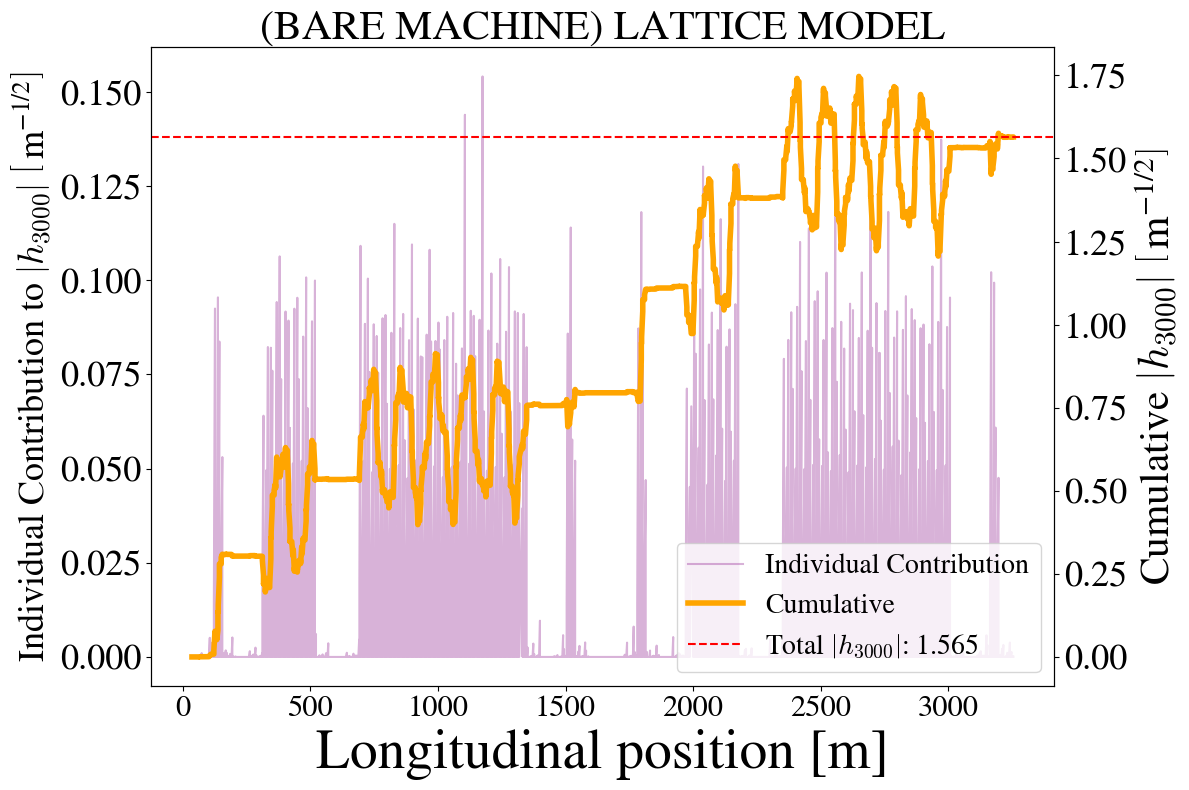
\includegraphics[width=\columnwidth]{chapter4/h3000_bare.png}
    \caption{Distribution of the $h_{3000}$ term around the ring with individual contributions from each relevant element and the cumulative sum from an arbitrary starting point.}
    \label{fig:h3000bare}
\end{figure}

\begin{figure}[H]
    \centering
    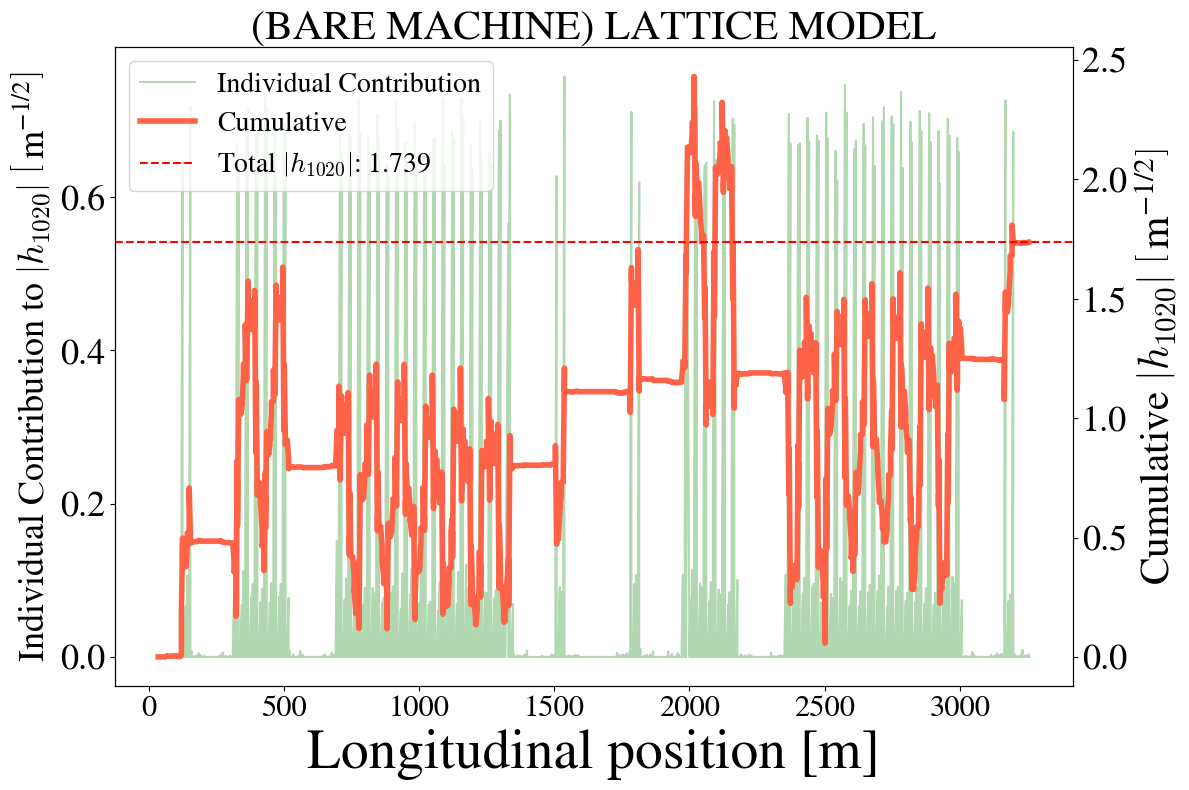
\includegraphics[width=\columnwidth]{chapter4/h1020_bare.png}
    \caption{Distribution of the $h_{1020}$ term around the ring with individual contributions from each relevant element and the cumulative sum from an arbitrary starting point.}
    \label{fig:h1020bare}
\end{figure}

\section{Measurement of Third Order RDTs}

\begin{equation}
    \label{eq:hxspect}
    h_x^{-}(N)= \hat{x} \pm \hat{p}_x = \sum_{jklm}HSL_{jklm}e^{2\pi i N \left[ \left( 1-j+k\right)Q_x+\left( m-l \right)Q_y\right]}
\end{equation}

\begin{equation}
    \label{eq:hyspect}
    h_y^{-}(N)= \hat{y} \pm \hat{p}_y = \sum_{jklm}VSL_{jklm}e^{2\pi i N \left[ \left( k-j\right)Q_x+\left(1-l+m \right)Q_y\right]}
\end{equation}

\begin{multline}
    \label{eq:hxpsi2}
    h_x^{-}(N)=\sqrt{2I_x}e^{i\left( \psi_x+\psi_{x_0}\right)} \\
    -2i \sum_{jklm} j f_{jklm} \left( 2I_x \right)^{\frac{j+k-1}{2}}\left( 2I_y \right)^{\frac{l+m}{2}}
    e^{i \left[ \left( 1-j+k\right)\left( \psi_x + \psi_{x_0} \right) +\left( m-l\right)\left( \psi_y + \psi_{y_0} \right)\right]}.
\end{multline}

\begin{multline}
    \label{eq:hypsi2}
    h_y^{-}(N)=\sqrt{2I_y}e^{i\left( \psi_y+\psi_{y_0}\right)} \\
    -2i \sum_{jklm} l f_{jklm} \left( 2I_x \right)^{\frac{j+k}{2}}\left( 2I_y \right)^{\frac{l+m-1}{2}}
    e^{i \left[ \left( k-j\right)\left( \psi_x + \psi_{x_0} \right) +\left( 1-l+m\right)\left( \psi_y + \psi_{y_0} \right)\right]}.
\end{multline}

\begin{figure}[H]
    \centering
    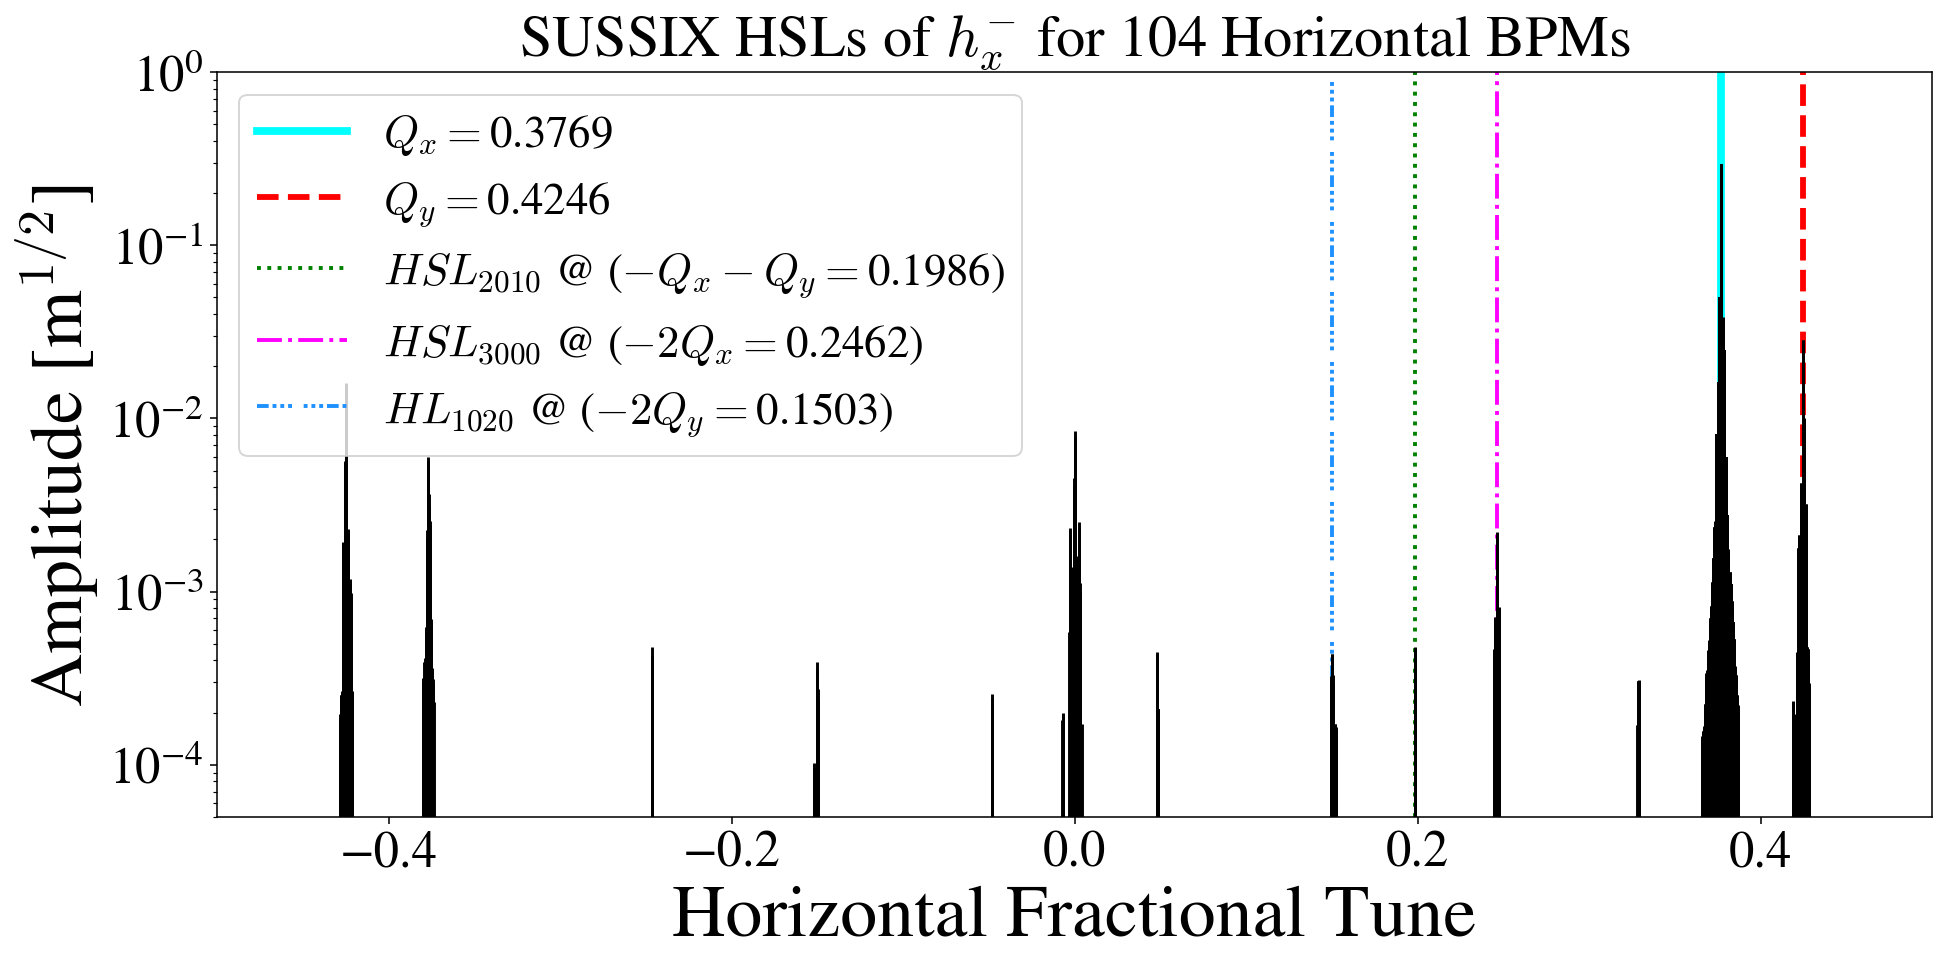
\includegraphics[width=\columnwidth]{chapter4/hxspect.png}
    \caption{Spectral lines of $h_x^{-}$ calculated with SUSSIX \cite{sussix}. The $h_x^{-}$ signal was reconstructed for the 104 Horizontal BPMs. The spectrum for all BPMs is superimposed in this plot.}
    \label{fig:hxspect1}
\end{figure}

\begin{figure}[H]
    \centering
    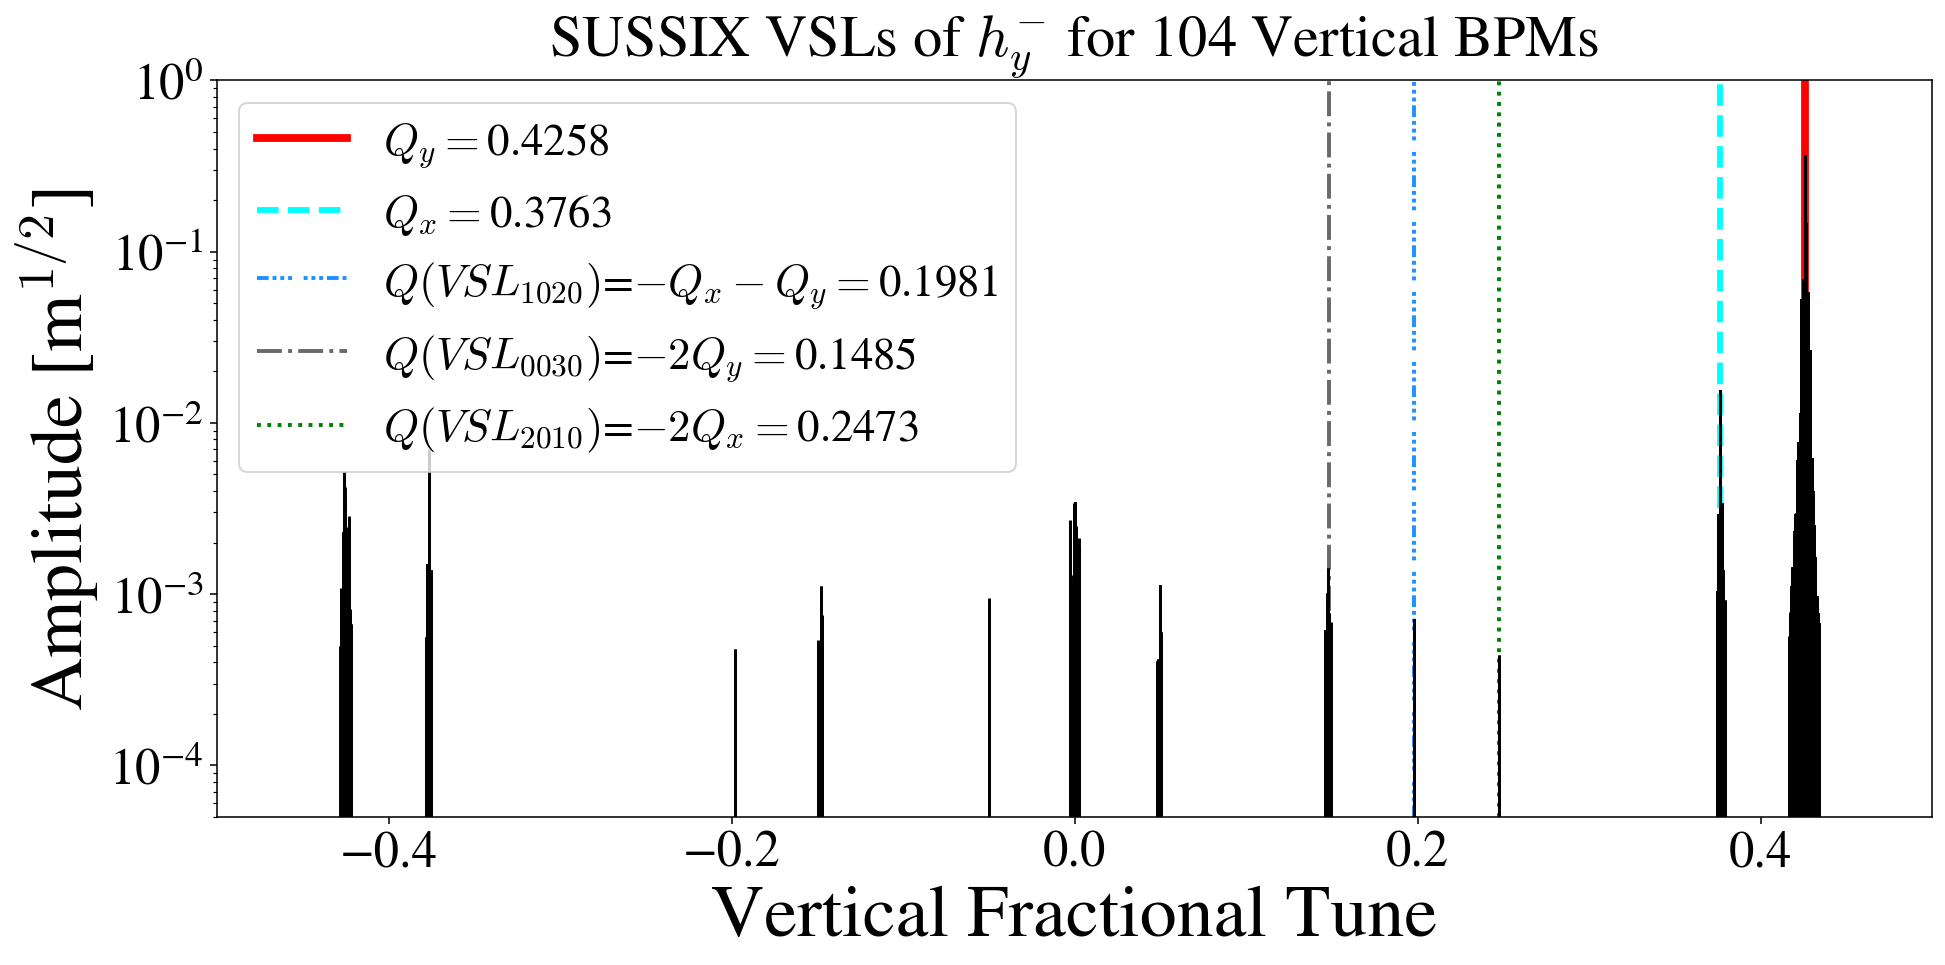
\includegraphics[width=\columnwidth]{chapter4/hyspect.png}
    \caption{Spectral lines of $h_y^{-}$ calculated with SUSSIX \cite{sussix}. The $h_y^{-}$ signal was reconstructed for the 104 Vertical BPMs. The spectrum for all BPMs is superimposed in this plot.}
    \label{fig:hyspect1}
\end{figure}

\begin{table}[H]
    \centering
    \caption{Corresponding RDTs and location of spectral lines for each resonance line.}
    \begin{tabular}{lcccc}
        \toprule
        \textbf{Resonance Line} & \textbf{Source} & \textbf{RDT} & \textbf{Hor. Spect.} & \textbf{Vert. Spect.} \\
        \midrule
            $3Q_x=76$     & Normal Sextupole    & $h_{3000}$           &  (-2,0)  & -       \\ %[3pt]
           $Q_x+2Q_y=74$   & Normal Sextupole    & $h_{1020}$            & (0,-2) & (-1,-1)       \\ %[3pt]
            $3Q_y=73$     & Skew Sextupole   & $h_{0030}$           & - & (0,-2)        \\ %[3pt]
            $2Q_x+Q_y=75$   & Skew Sextupole    & $h_{2010}$     & (-1,-1) & (-2,0)       \\
        \bottomrule
    \end{tabular}
    \label{tab:rdtlines}
\end{table}

\begin{figure}[H]
    \centering
    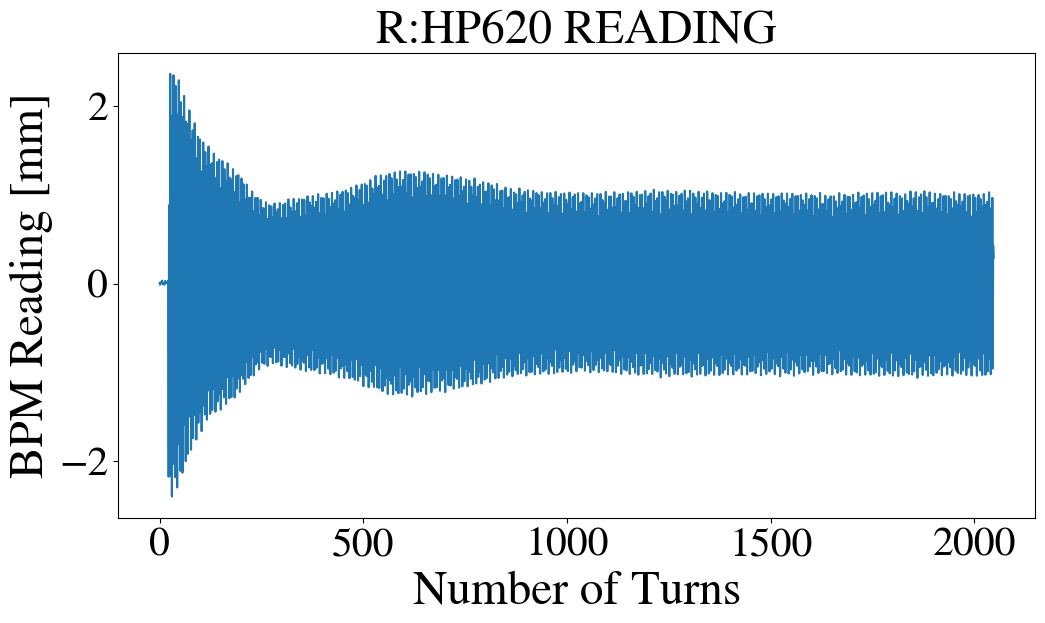
\includegraphics[width=\columnwidth]{chapter4/bpm_kick.png}
    \caption{}
    \label{fig:bpm_kick0}
\end{figure}

\begin{figure}[H]
    \centering
    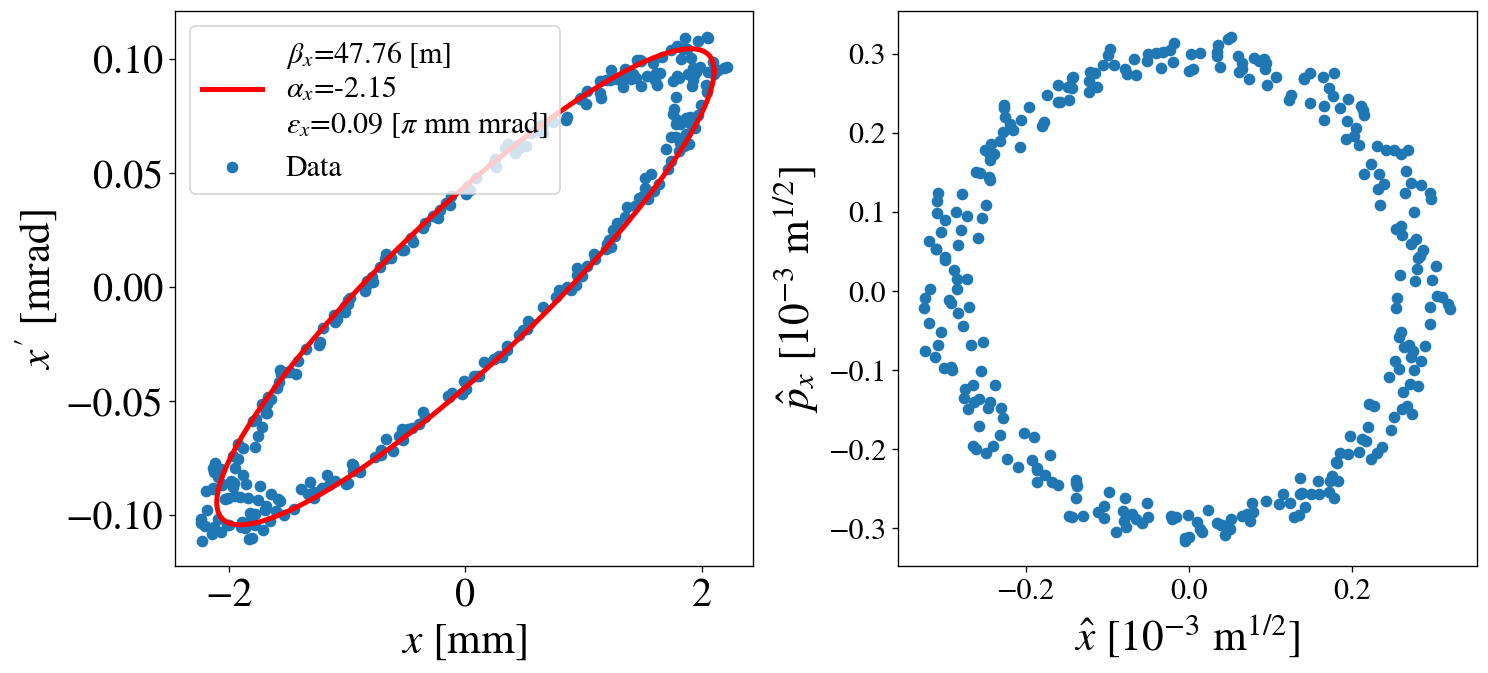
\includegraphics[width=\columnwidth]{chapter4/ellipse_data.png}
    \caption{}
    \label{fig:ellipse}
\end{figure}

\section{Compensation of RDTs}

\begin{equation}
    \begin{bmatrix}
        -|{h_{3000}}|  \cos (\psi_{3000})\\
        -|{h_{3000}}|  \sin (\psi_{3000})\\
        -|{h_{1020}}|  \cos (\psi_{1020})\\
        -|{h_{1020}}|  \sin (\psi_{1020})\\
      \end{bmatrix}_{(Bare)}
    =
      \boldsymbol{M}
    \begin{bmatrix}
        I_{sc220} \\
        I_{sc222} \\
        I_{sc319} \\
        I_{sc321} \\
      \end{bmatrix}
\end{equation}

\begin{equation}
    \begin{bmatrix}
        -|{h_{3000}}|  \cos (\psi_{3000})\\
        -|{h_{3000}}|  \sin (\psi_{3000})\\
        -|{h_{1020}}|  \cos (\psi_{1020})\\
        -|{h_{1020}}|  \sin (\psi_{1020})\\
        -|{h_{0030}}|  \cos (\psi_{3000})\\
        -|{h_{0030}}|  \sin (\psi_{3000})\\
        -|{h_{2010}}|  \cos (\psi_{1020})\\
        -|{h_{2010}}|  \sin (\psi_{1020})\\
      \end{bmatrix}_{(Bare)}
    =
      \boldsymbol{M}
    \begin{bmatrix}
        I_{sc220} \\
        I_{sc222} \\
        I_{sc319} \\
        I_{sc321} \\
        I_{ss223} \\
        I_{ss323} \\
        I_{ss319} \\
        I_{ss321} \\
      \end{bmatrix}
\end{equation}
 
\begin{equation}
    \begin{bmatrix}
        -|h_{3000}| \cos \psi_{3000} \\
        -|h_{3000}| \sin \psi_{3000} \\
        -|h_{1020}| \cos \psi_{1020} \\
        -|h_{1020}| \sin \psi_{1020} \\
        \end{bmatrix}_{(Bare)}
         =
        \boldsymbol{M}
        \begin{bmatrix}
        k_2^{(sc220)} \\
        k_2^{(sc222)}\\
        k_2^{(sc319)} \\
        k_2^{(sc321)}\\
        k_2^{(1)} \\
        k_2^{(2)}\\
        \end{bmatrix}
\end{equation}

\begin{equation}
    \begin{bmatrix}
        -|h_{3000}| \cos \psi_{3000} \\
        -|h_{3000}| \sin \psi_{3000} \\
        -|h_{1020}| \cos \psi_{1020} \\
        -|h_{1020}| \sin \psi_{1020} \\
        \end{bmatrix}_{(Bare)}
         =
        \boldsymbol{M}
        \begin{bmatrix}
        k_2^{(sc220)} \\
        k_2^{(sc222)}\\
        k_2^{(sc319)} \\
        k_2^{(sc321)}\\
        \end{bmatrix}        
\end{equation}

\begin{figure}[H]
    \centering
    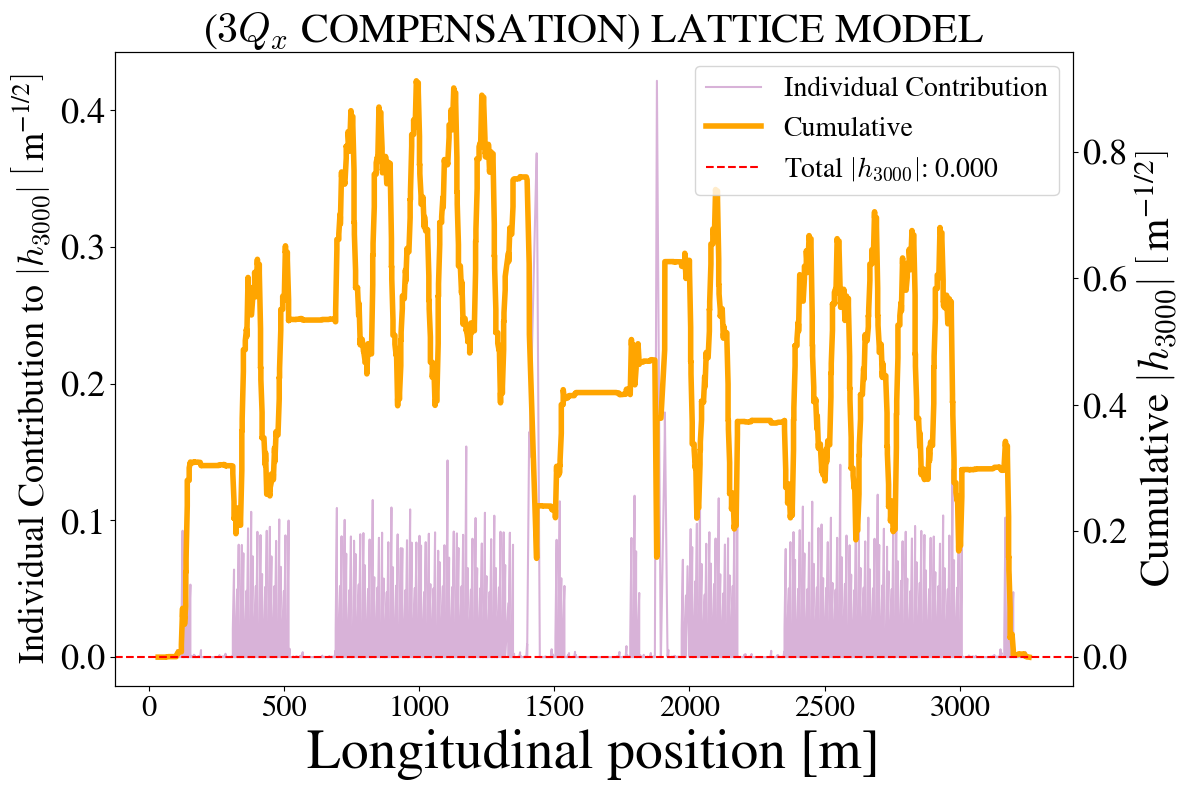
\includegraphics[width=\columnwidth]{chapter4/h3000_3qxcomp.png}
    \caption{Distribution of the $h_{3000}$ term around the ring with individual contributions from each relevant element and the cumulative sum from an arbitrary starting point when correction elements are set to compensate $3Q_x=76$, i.e., $h_{3000}=0$.}
    \label{fig:h3000_3qxcomp}
\end{figure}

\begin{figure}[H]
    \centering
    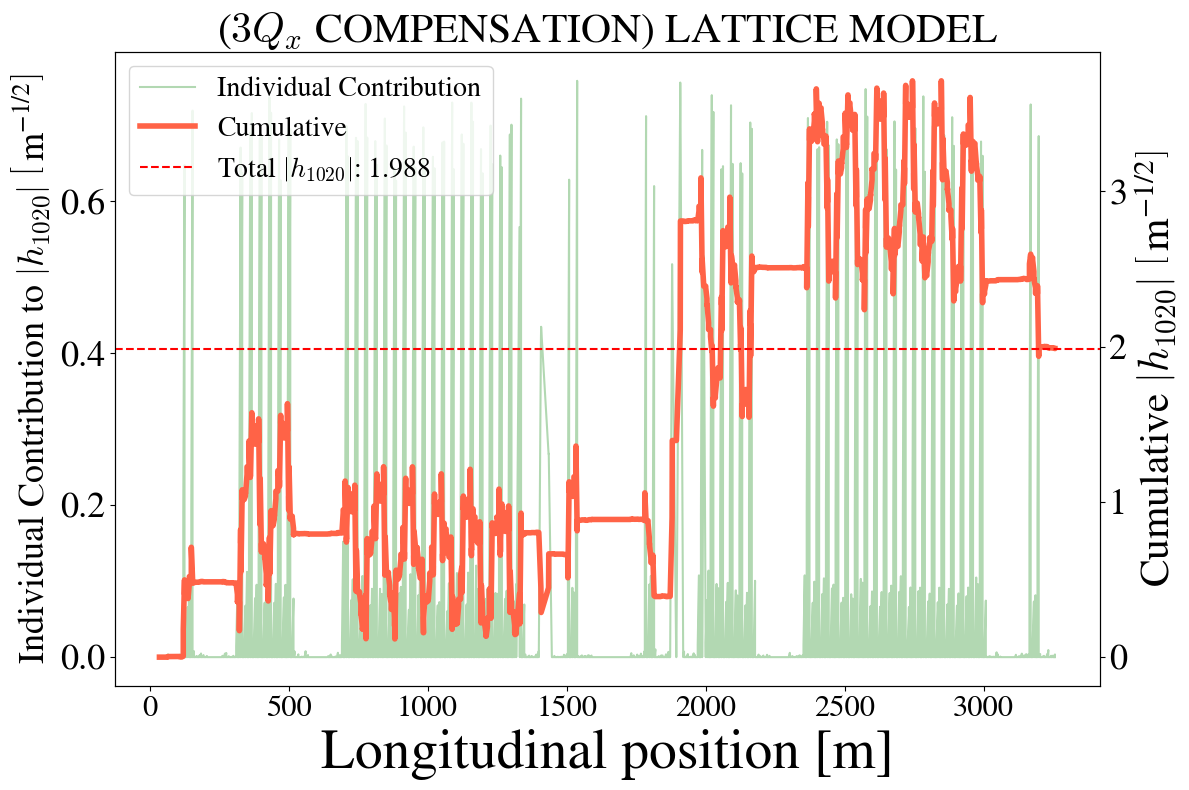
\includegraphics[width=\columnwidth]{chapter4/h1020_3qxcomp.png}
    \caption{Distribution of the $h_{3000}$ term around the ring with individual contributions from each relevant element and the cumulative sum from an arbitrary starting point when correction elements are set to compensate $3Q_x=76$, i.e., $h_{3000}=0$.}
    \label{fig:h1020_3qxcomp}
\end{figure}

\section{Optimization of Compensation Currents}

\section{Experimental Verification of Compensation}

\subsection{\label{sec:lossmaps}Dynamic Loss Maps}

\begin{figure}[H]
    \centering
    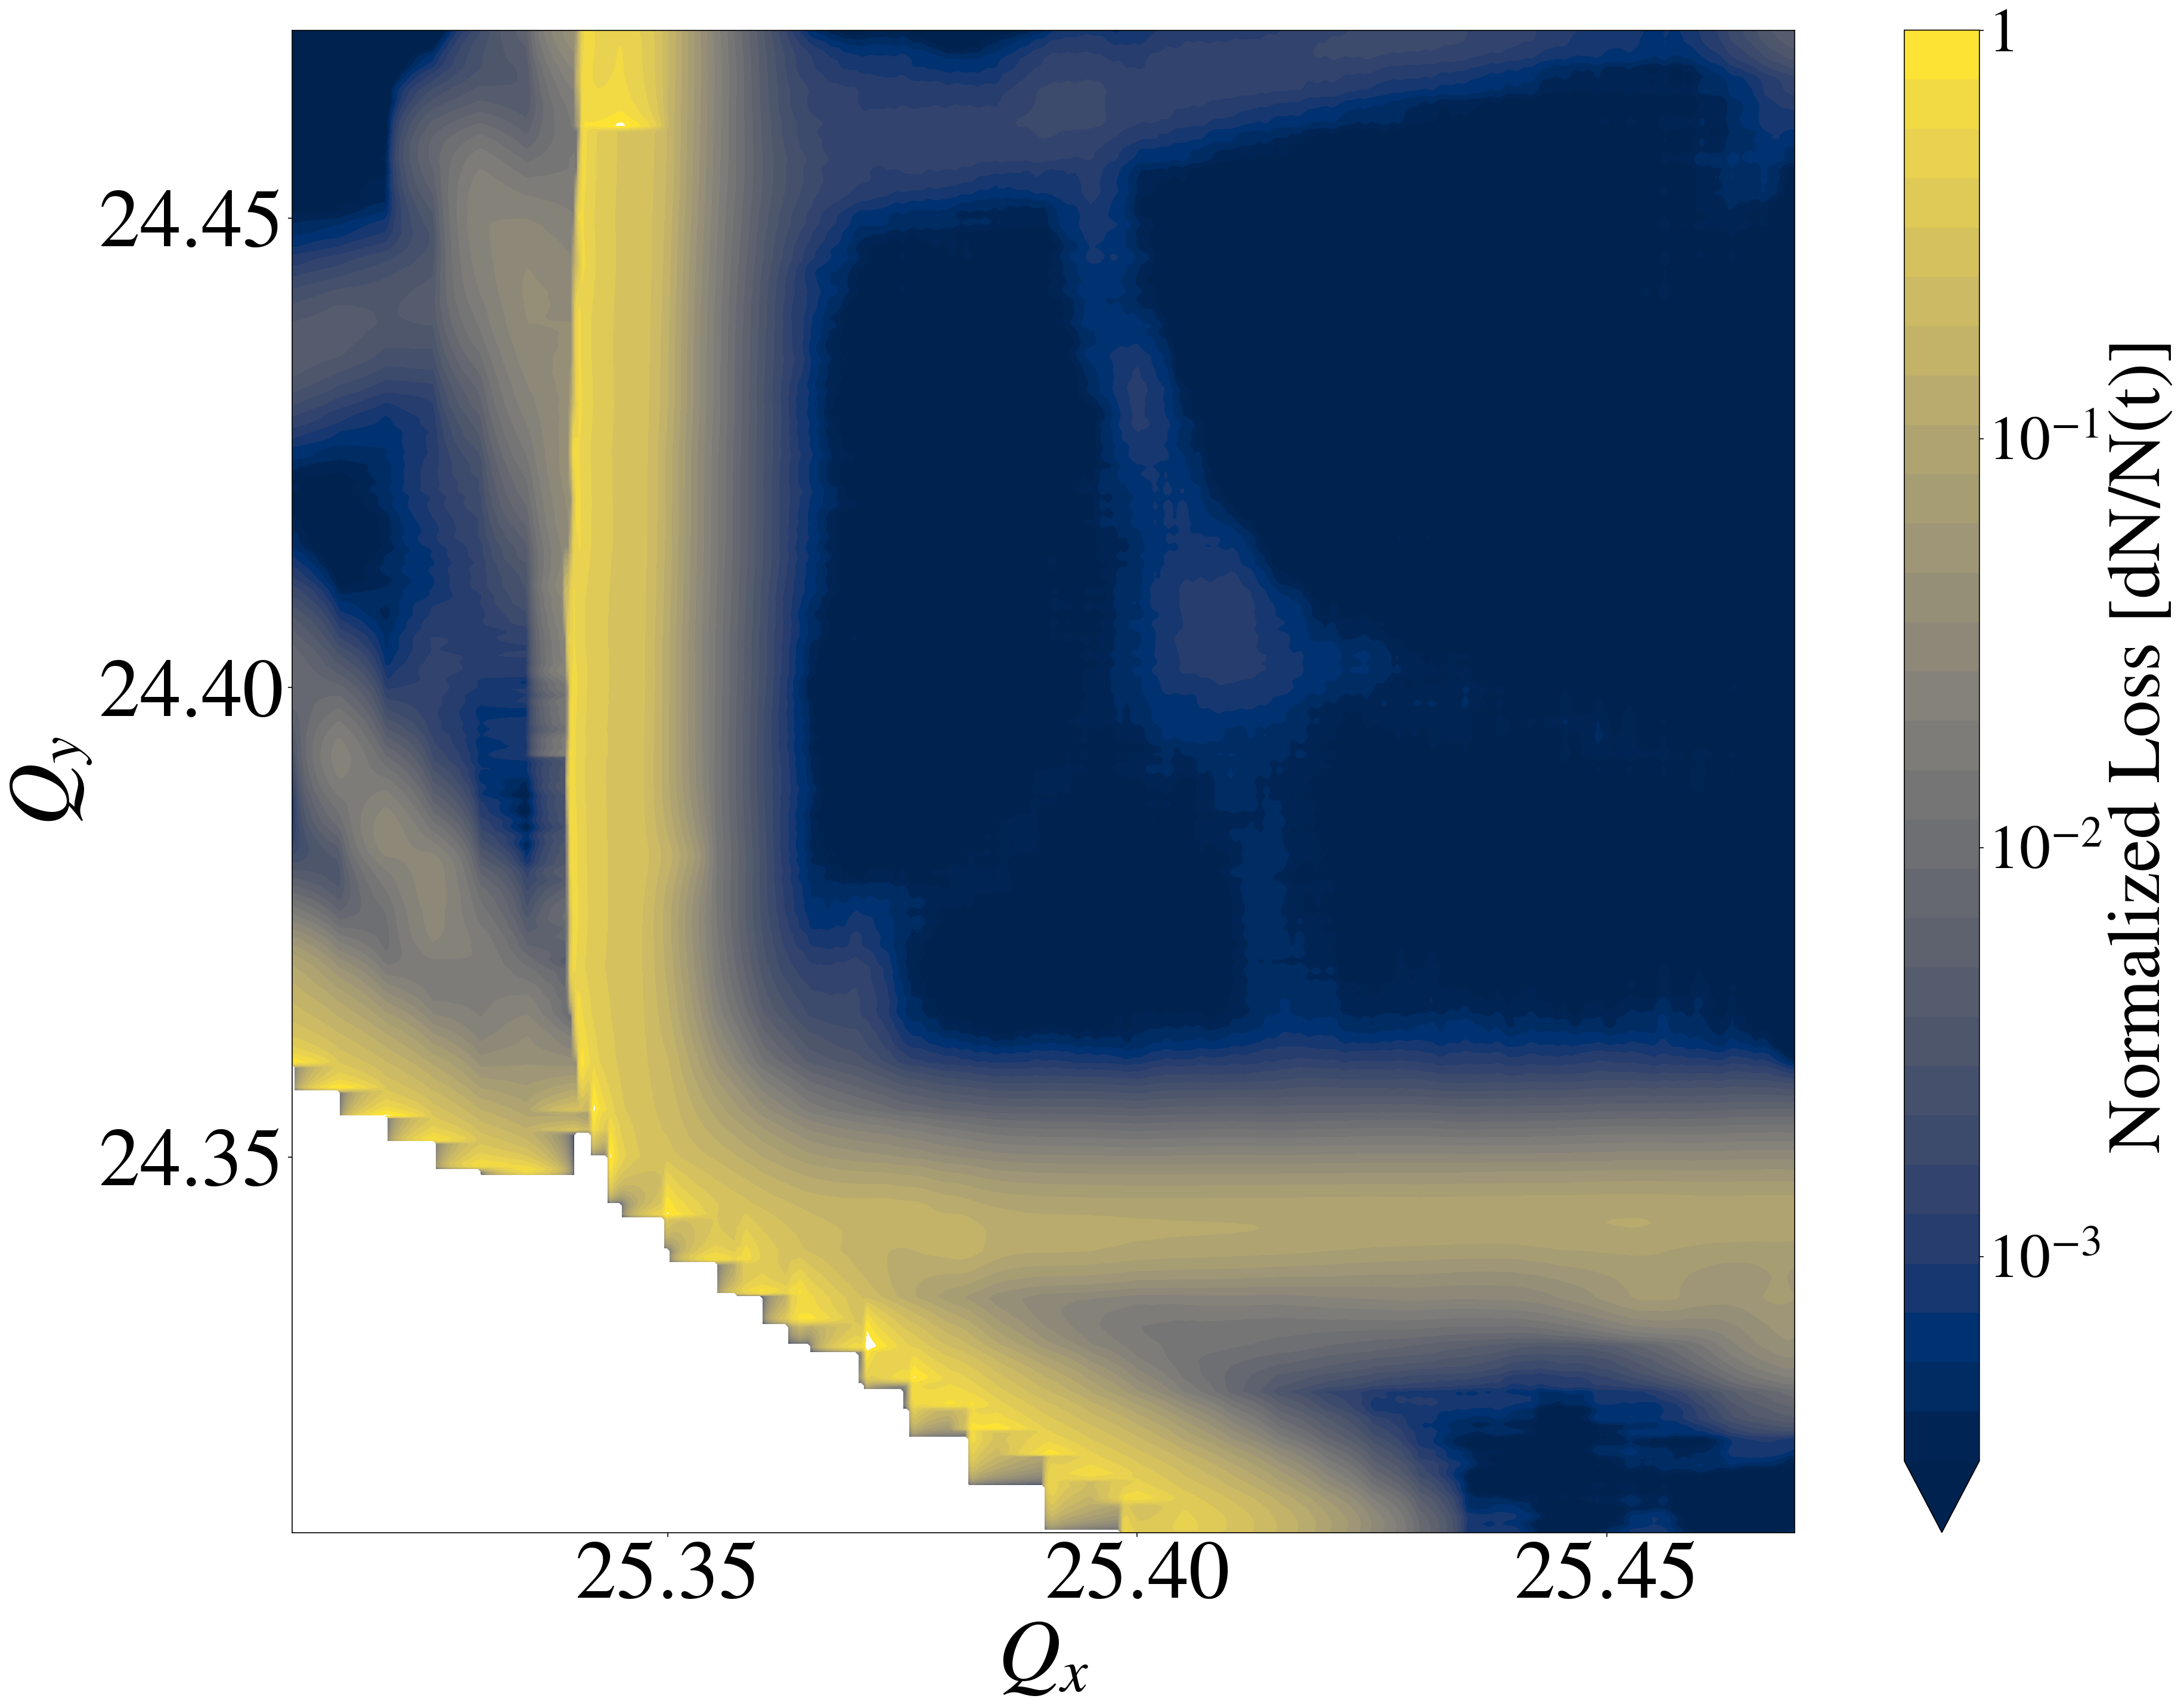
\includegraphics[width=\columnwidth]{chapter4/bare.png}
    \caption{Dynamic loss map from ramping the tunes with an interval of $\Delta Q_u=0.005$ in both directions. The directions of scan are from left to right and top to bottom. The results are superimposed in this plot.}
    \label{fig:bare_nocomments}
\end{figure}

\begin{figure}[H]
    \centering
    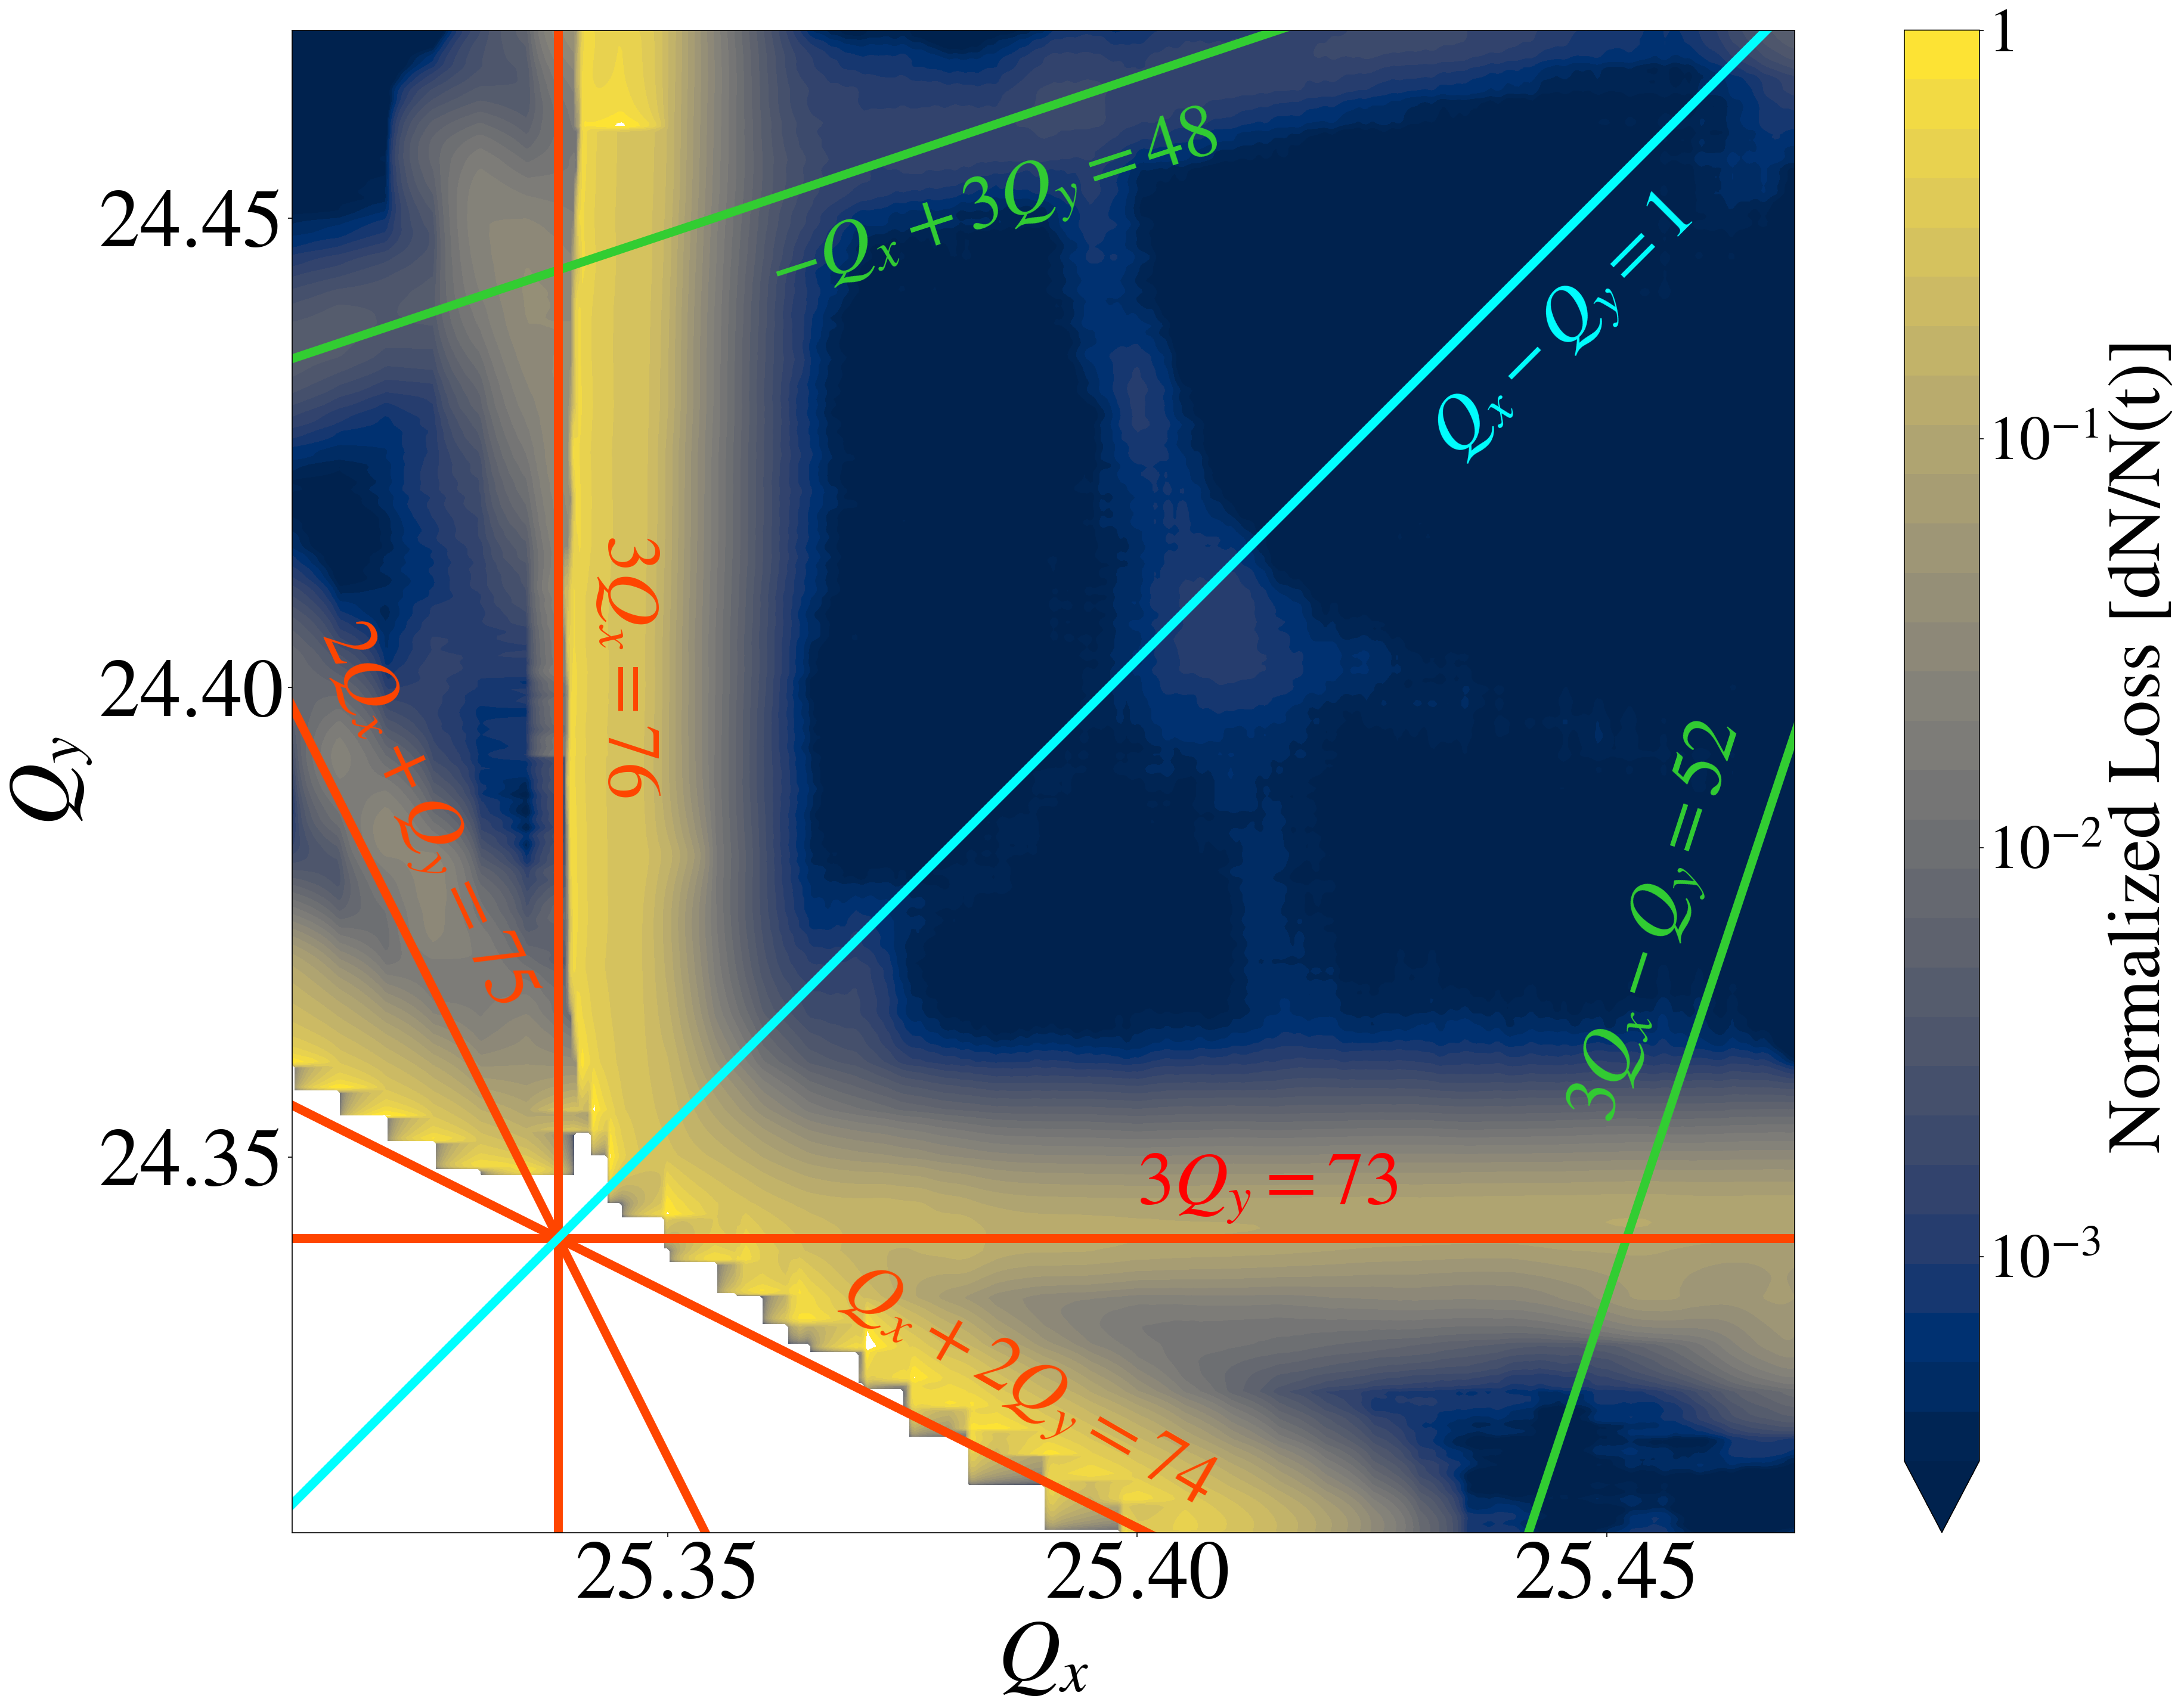
\includegraphics[width=\columnwidth]{chapter4/bare_comments.png}
    \caption{Dynamic loss map with the corresponding lines from Fig. \ref{fig:rrtd} drawn on top.}
    \label{fig:bare_comments}
\end{figure}


\newpage
\begin{figure}[H]

    \centering
    \begin{subfigure}{.49\textwidth}
      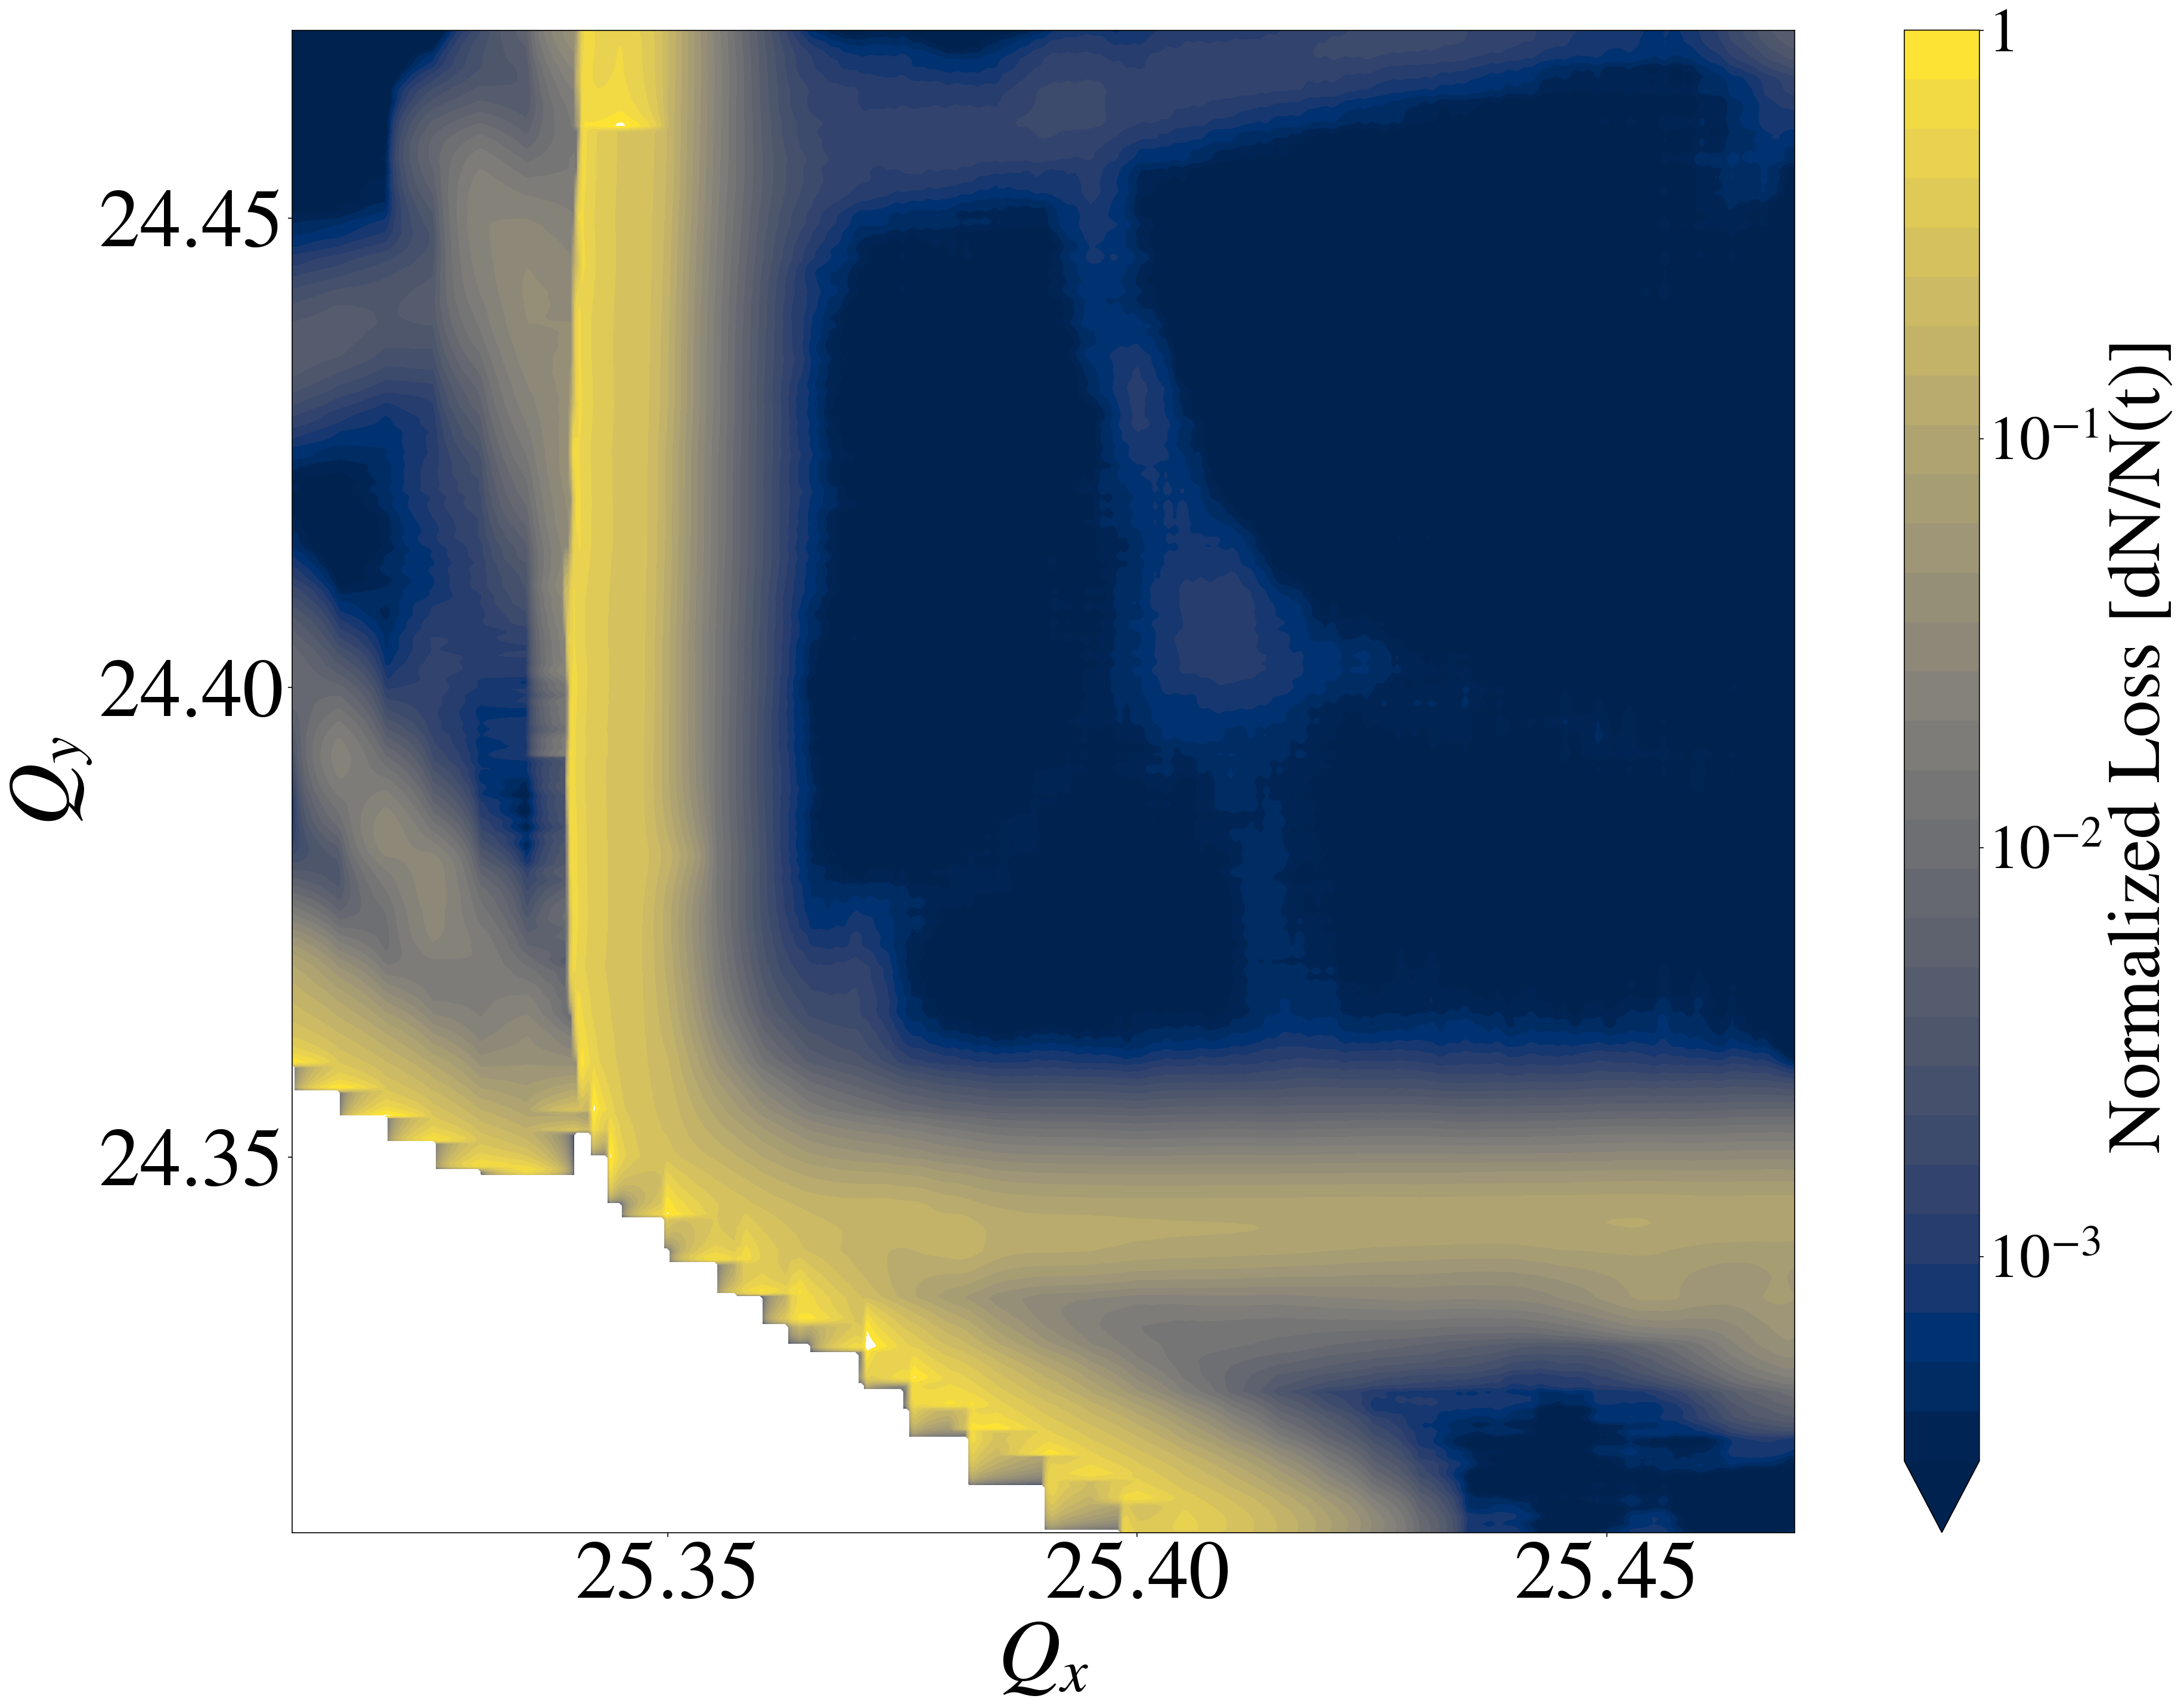
\includegraphics[width=0.98\linewidth]{chapter4/bare.png}
      \caption{Bare machine}
      \label{fig:sfig1}
    \end{subfigure}%
    \hfill
    \begin{subfigure}{.49\textwidth}
      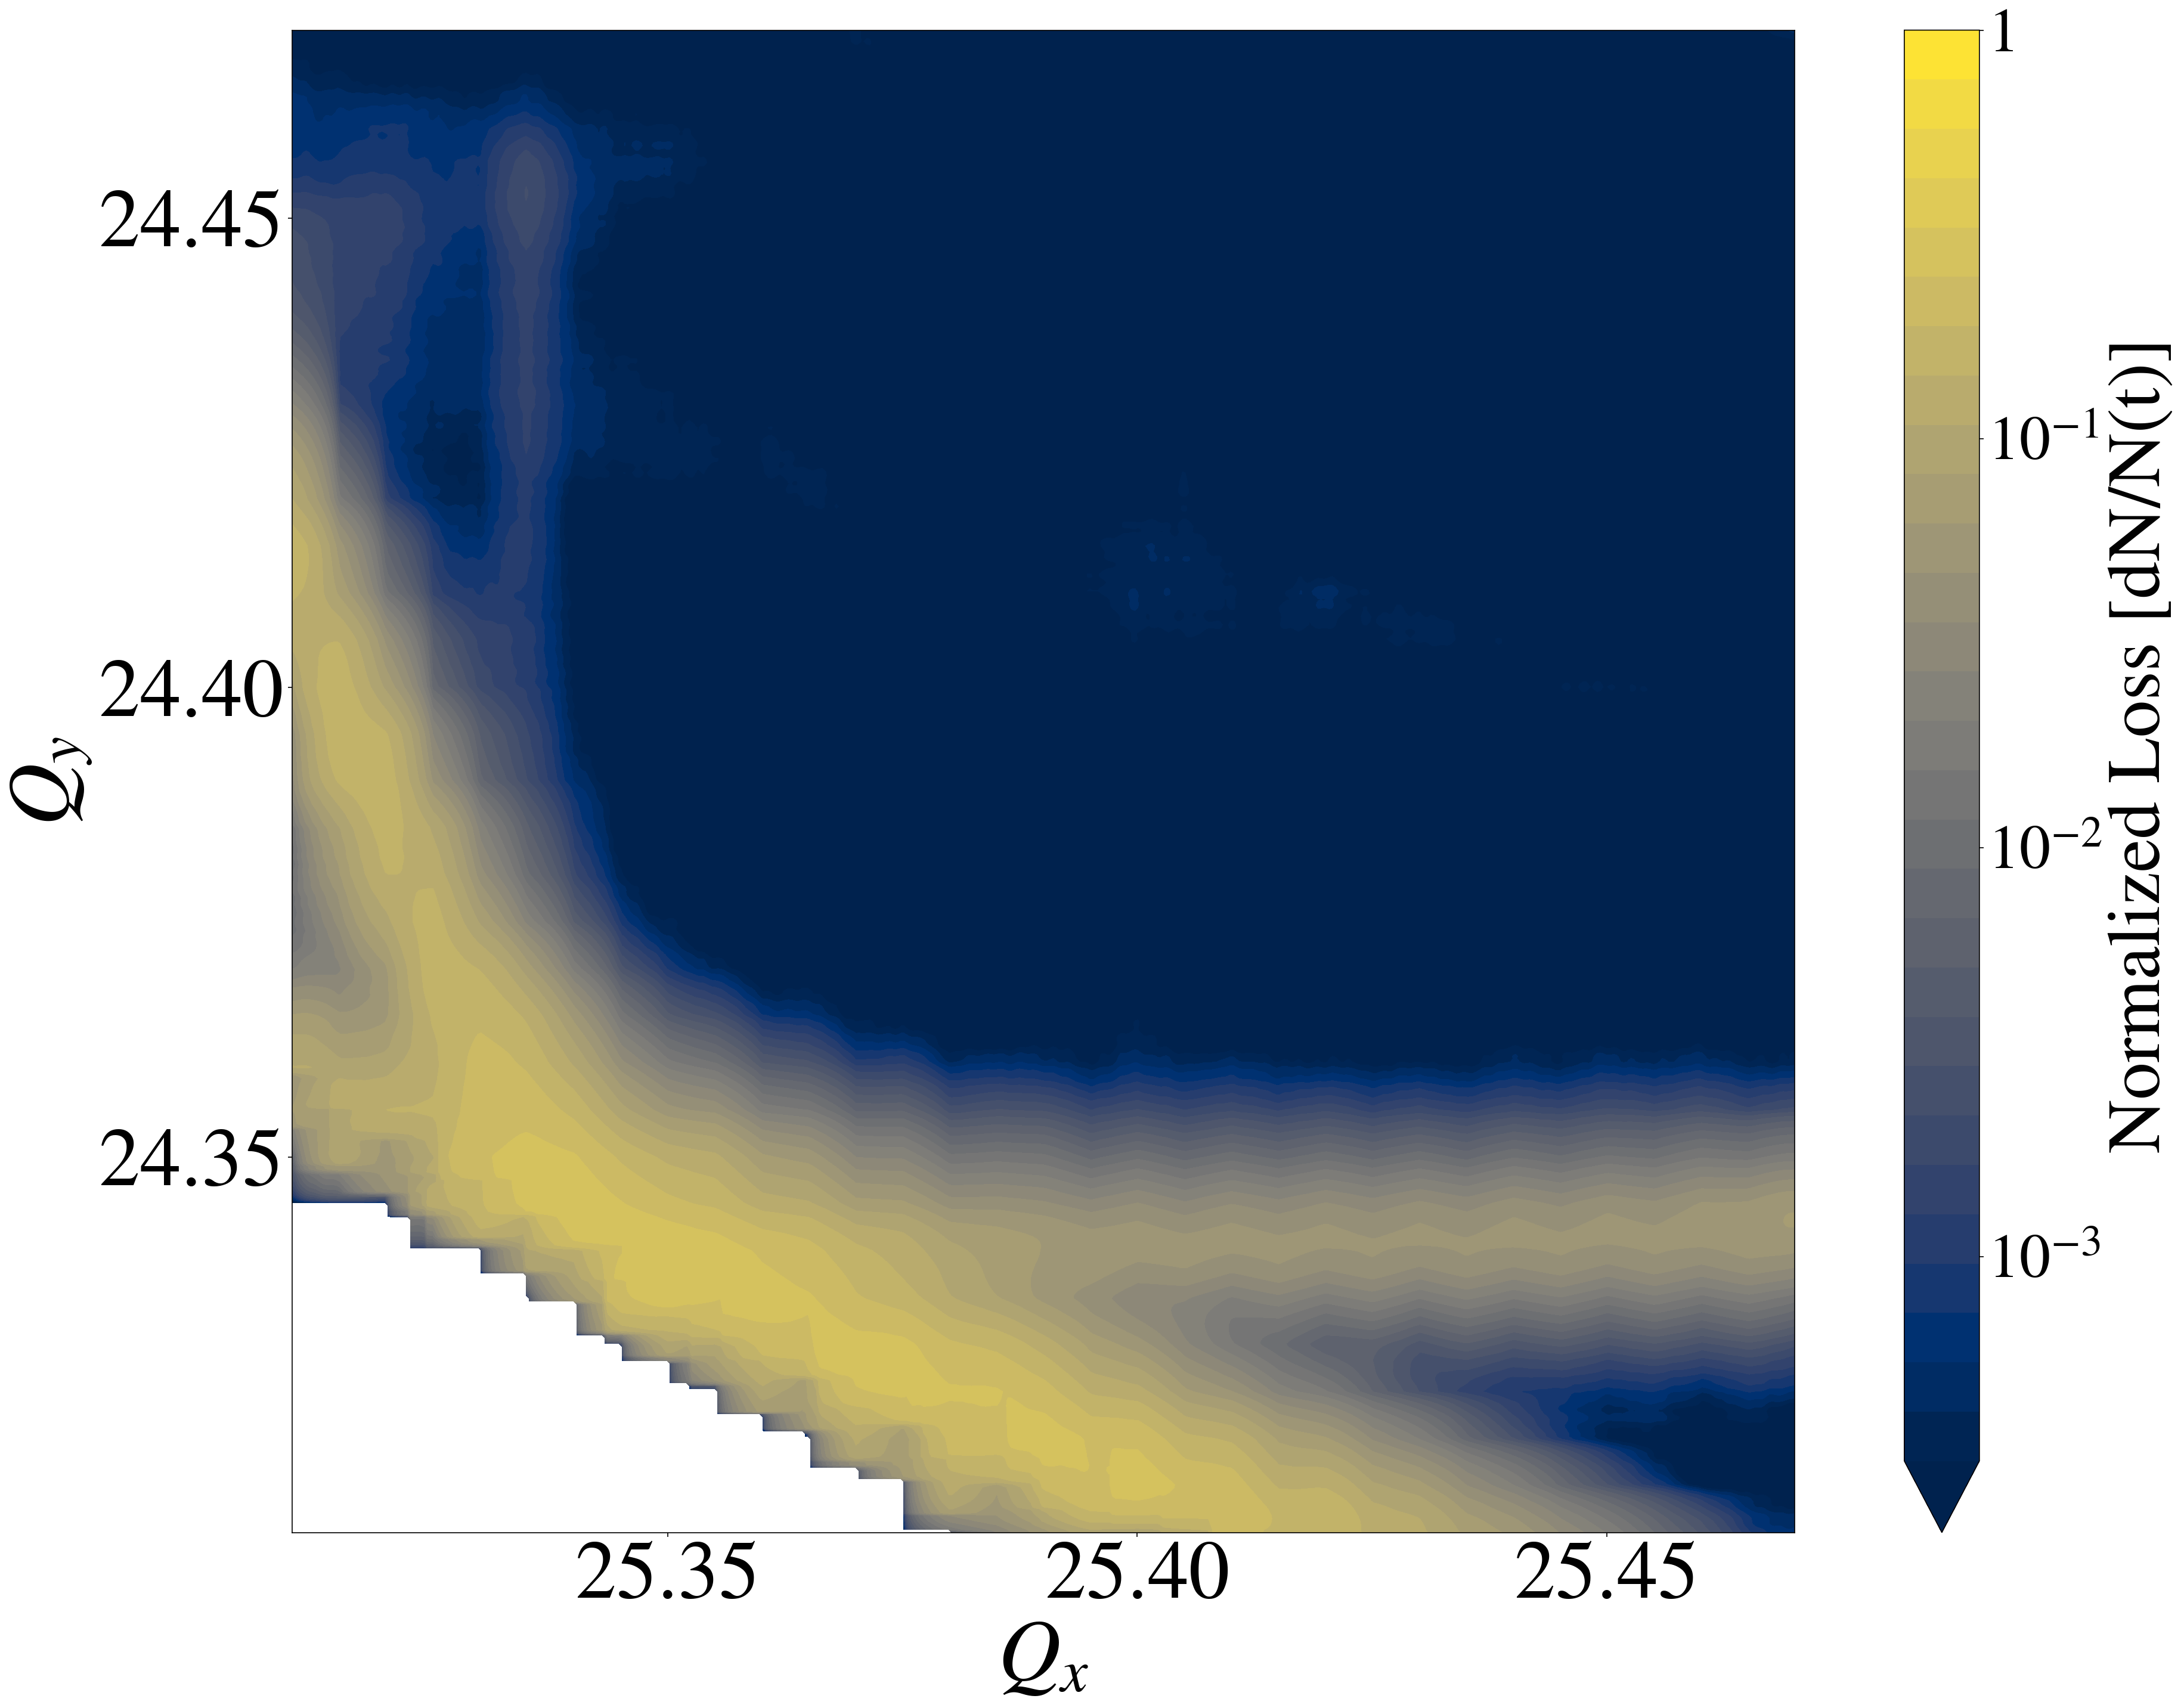
\includegraphics[width=0.98\linewidth]{chapter4/3qx.png}
      \caption{$3Q_x$ Compensation}
      \label{fig:sfig2}
    \end{subfigure}
    \hfill
    \begin{subfigure}{.49\textwidth}
      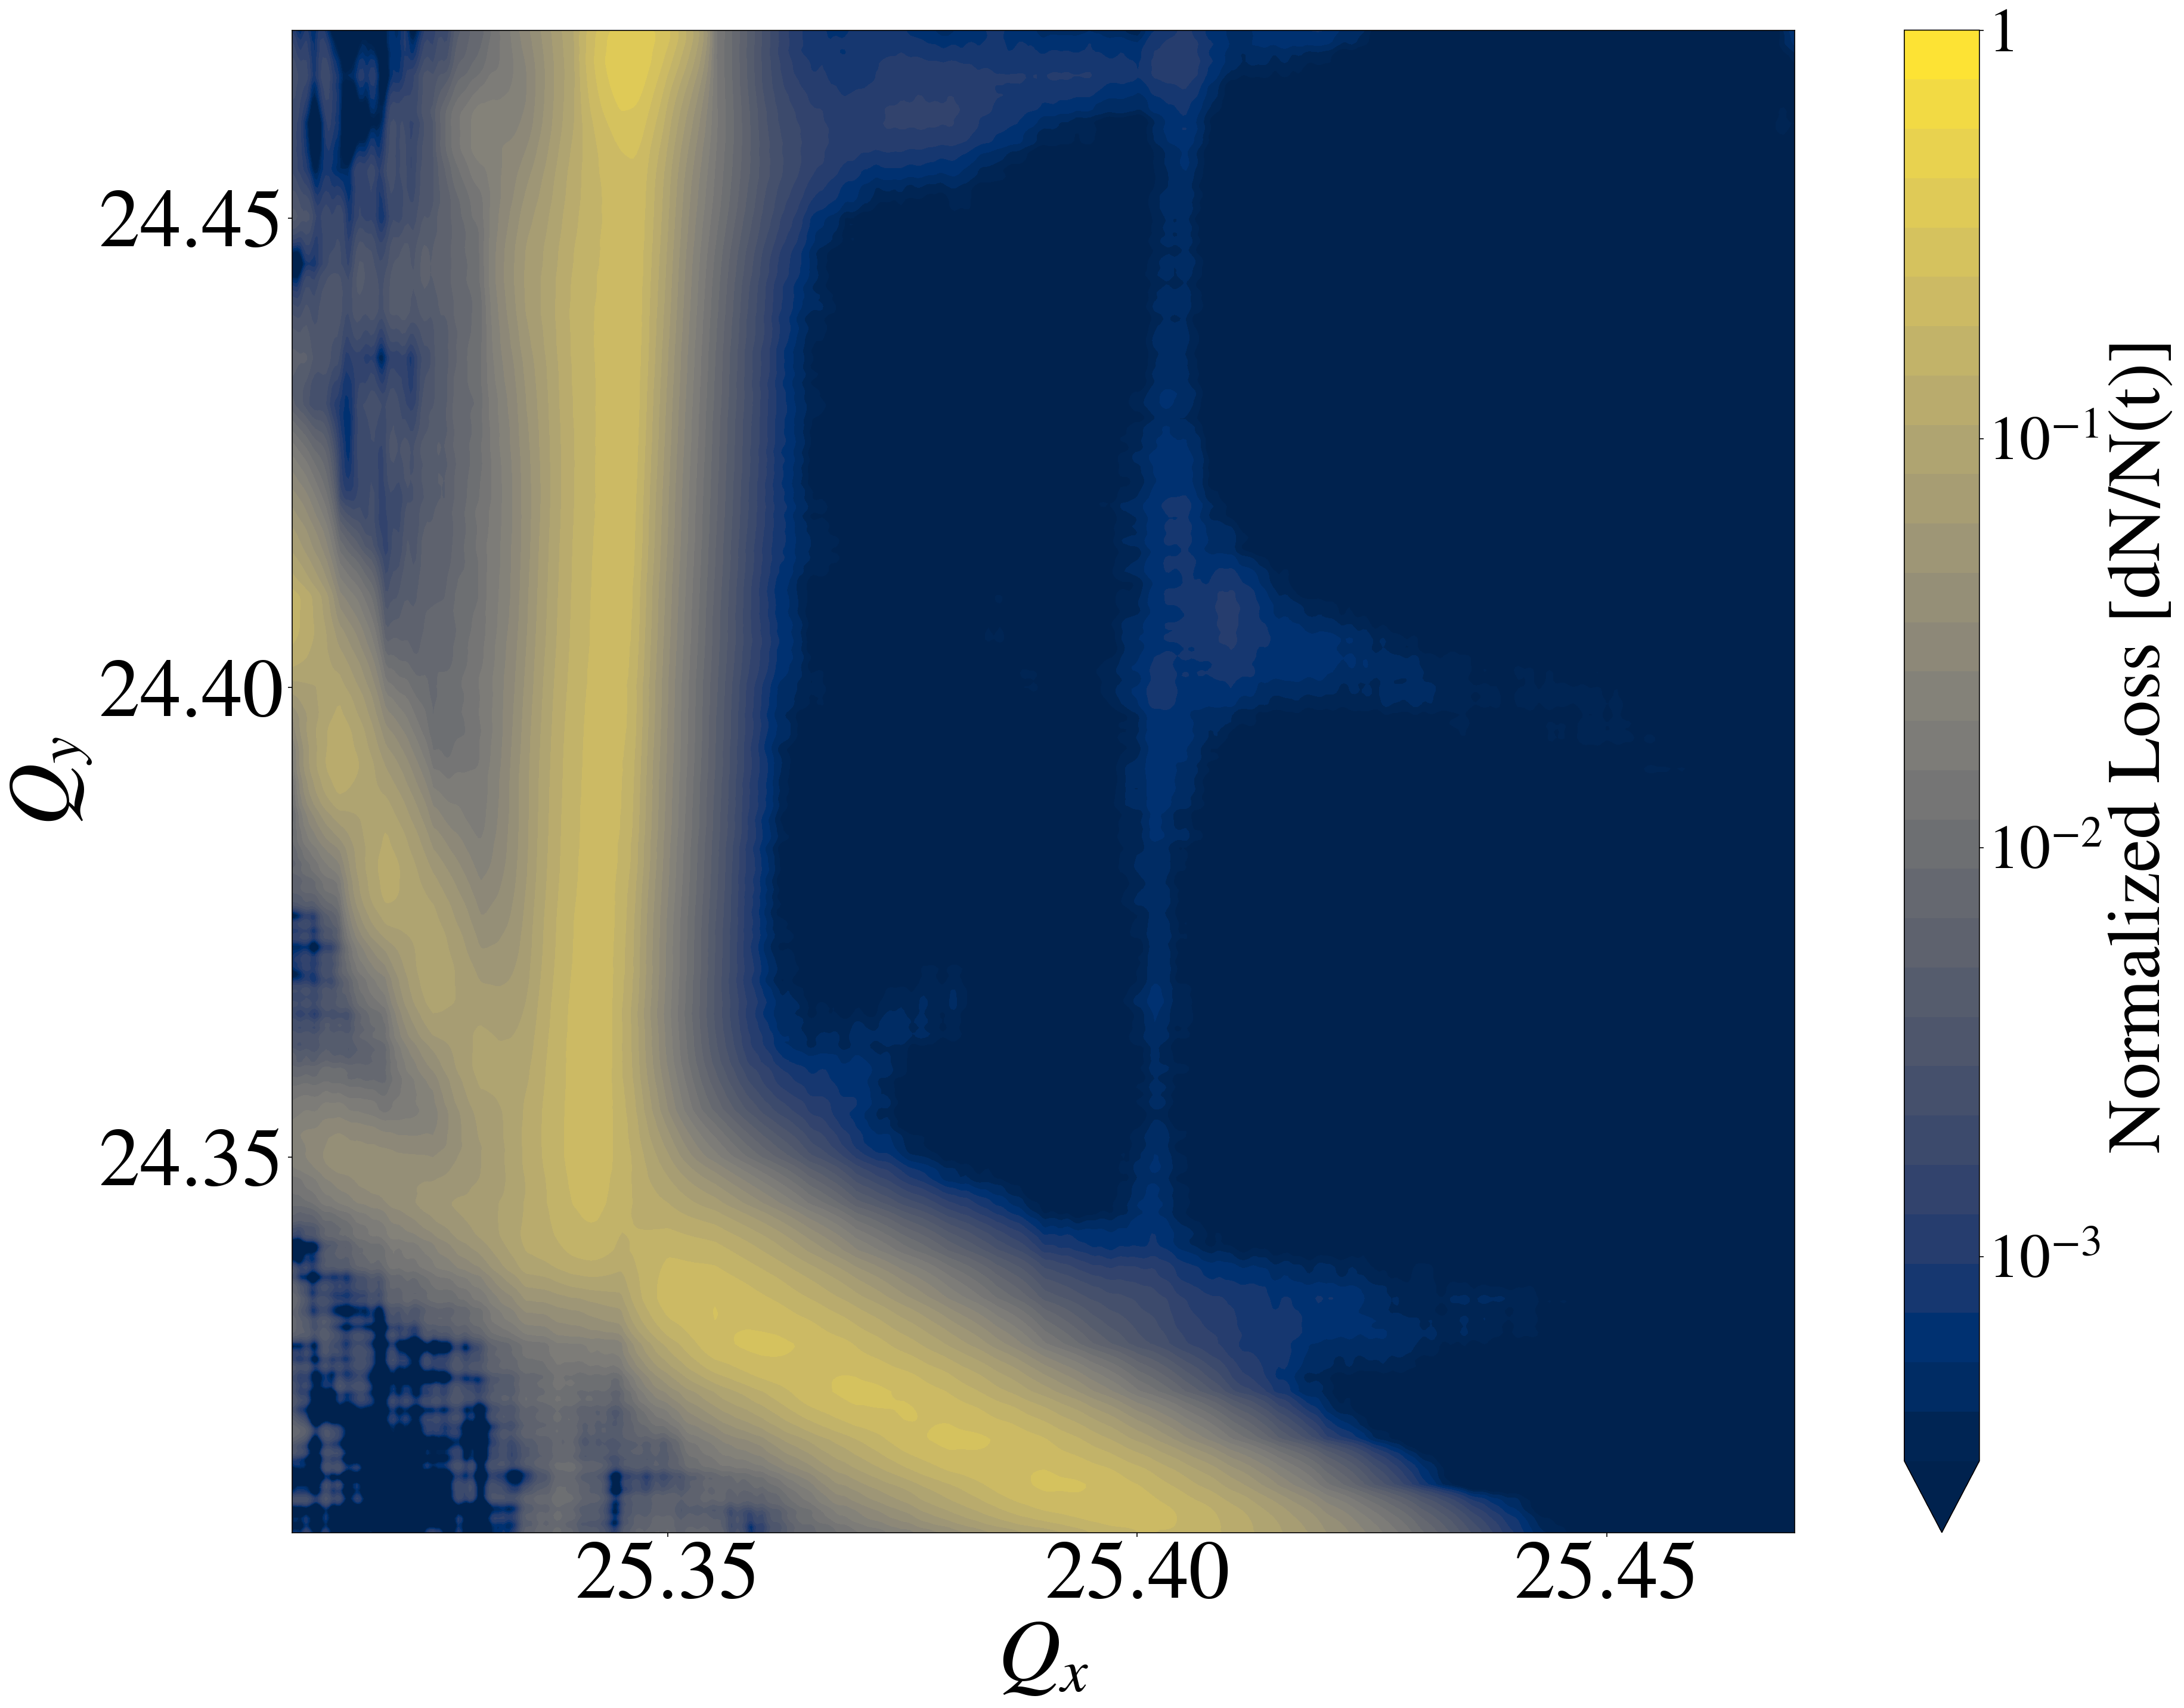
\includegraphics[width=0.98\linewidth]{chapter4/3qy.png}
      \caption{$3Q_y$ Compensation}
      \label{fig:sfig3}
    \end{subfigure}
    \hfill
    \begin{subfigure}{.49\textwidth}
      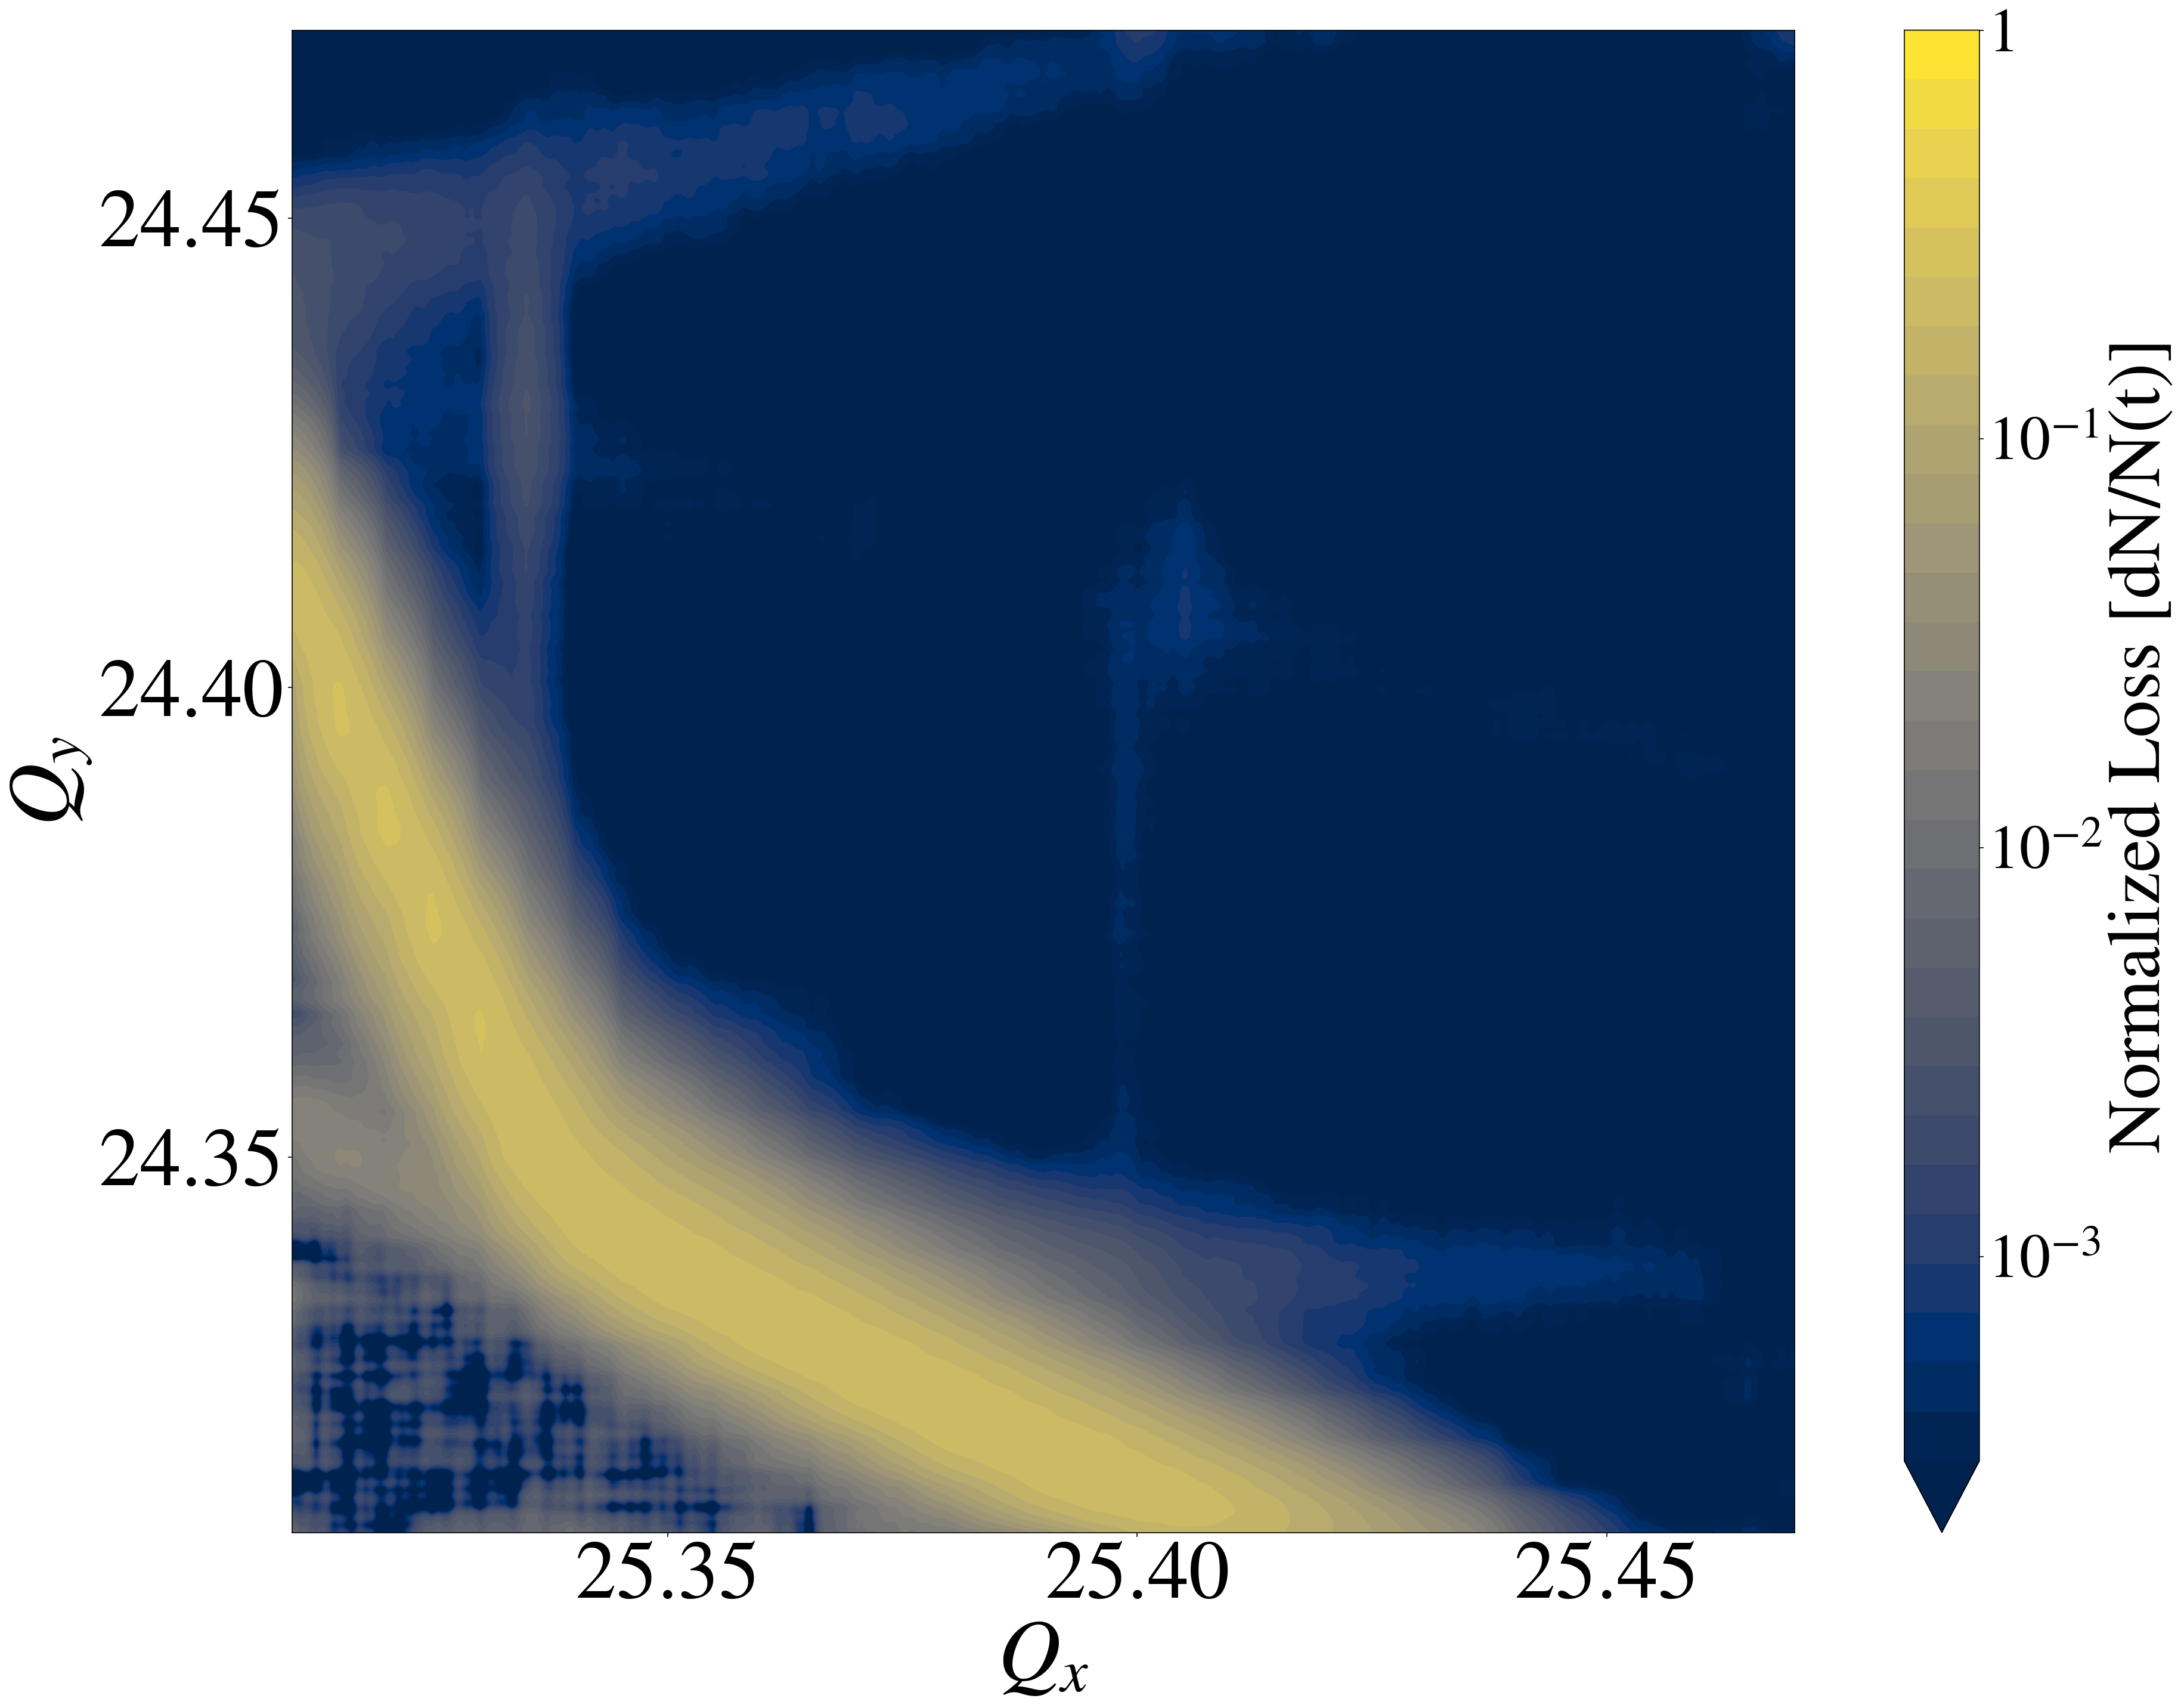
\includegraphics[width=0.98\linewidth]{chapter4/3qx_3qy.png}
      \caption{$3Q_x$ and $3Q_y$ Compensation}
      \label{fig:sfig4}
    \end{subfigure}%
    \hfill
    \begin{subfigure}{.49\textwidth}
      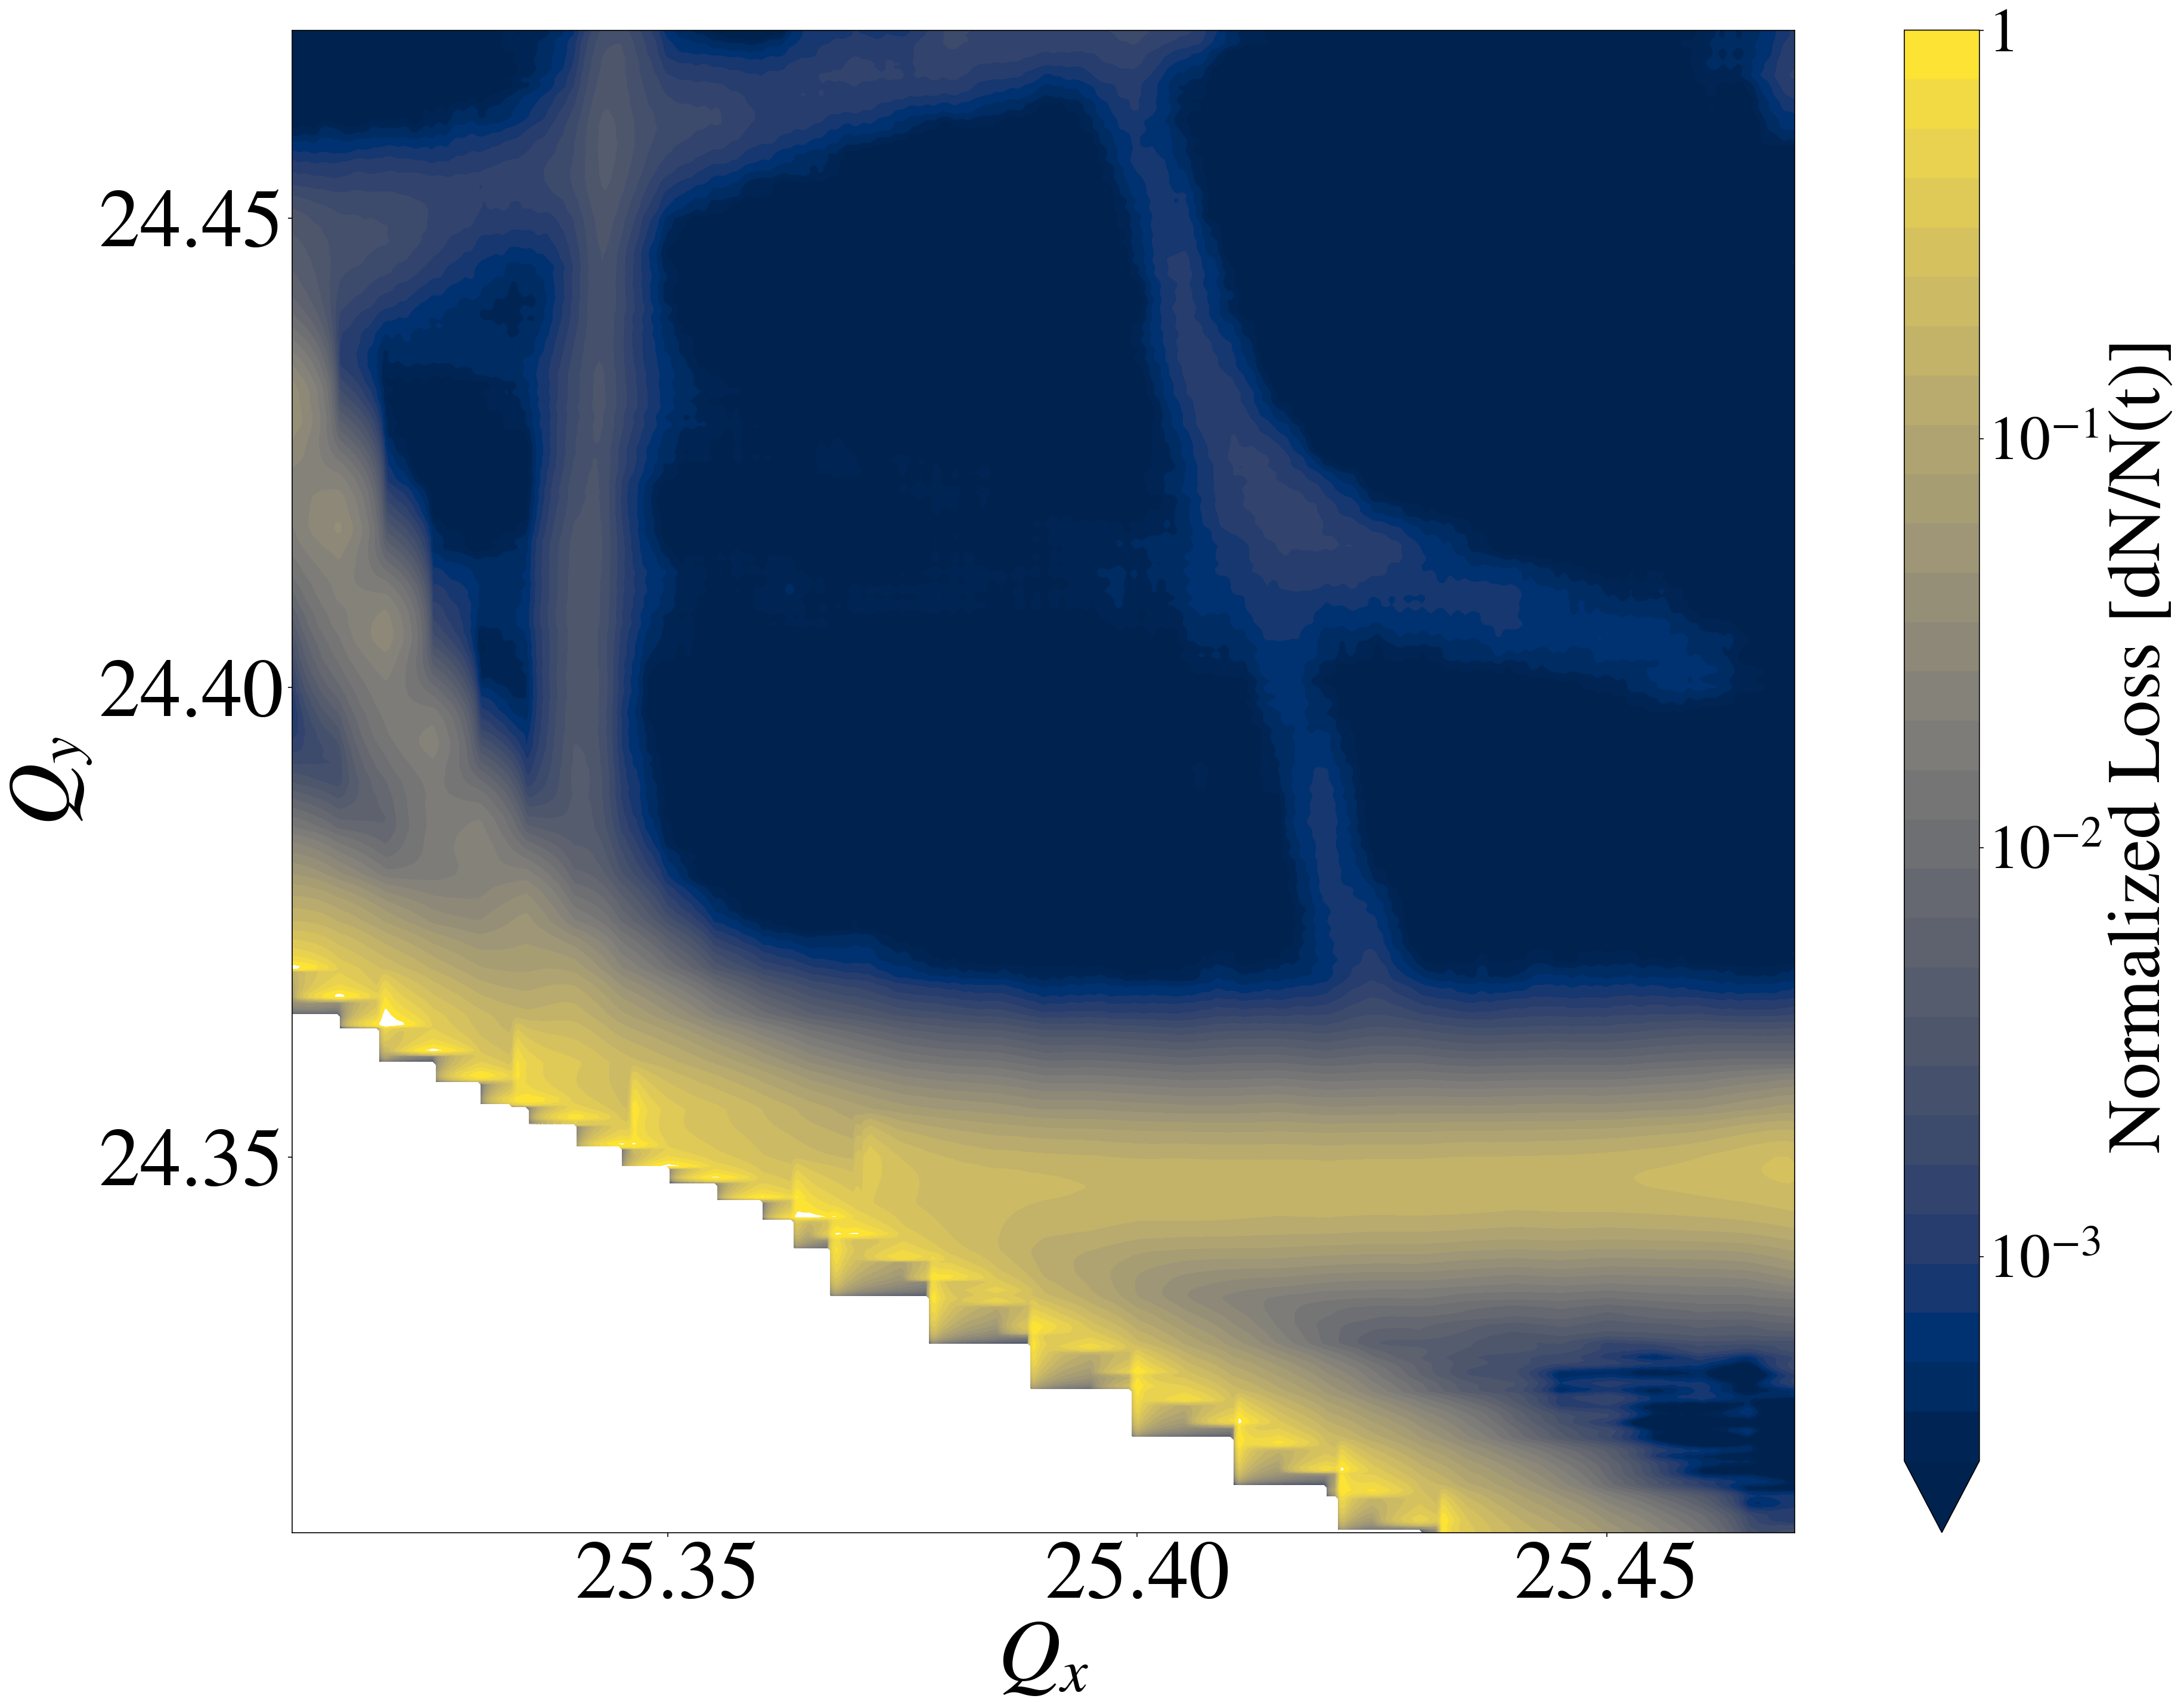
\includegraphics[width=0.98\linewidth]{chapter4/3qx_2qxqy.png}
      \caption{$3Q_x$ and $2Q_x+Q_y$ Compensation}
      \label{fig:sfig5}
    \end{subfigure}
    \hfill
    \begin{subfigure}{.49\textwidth}
      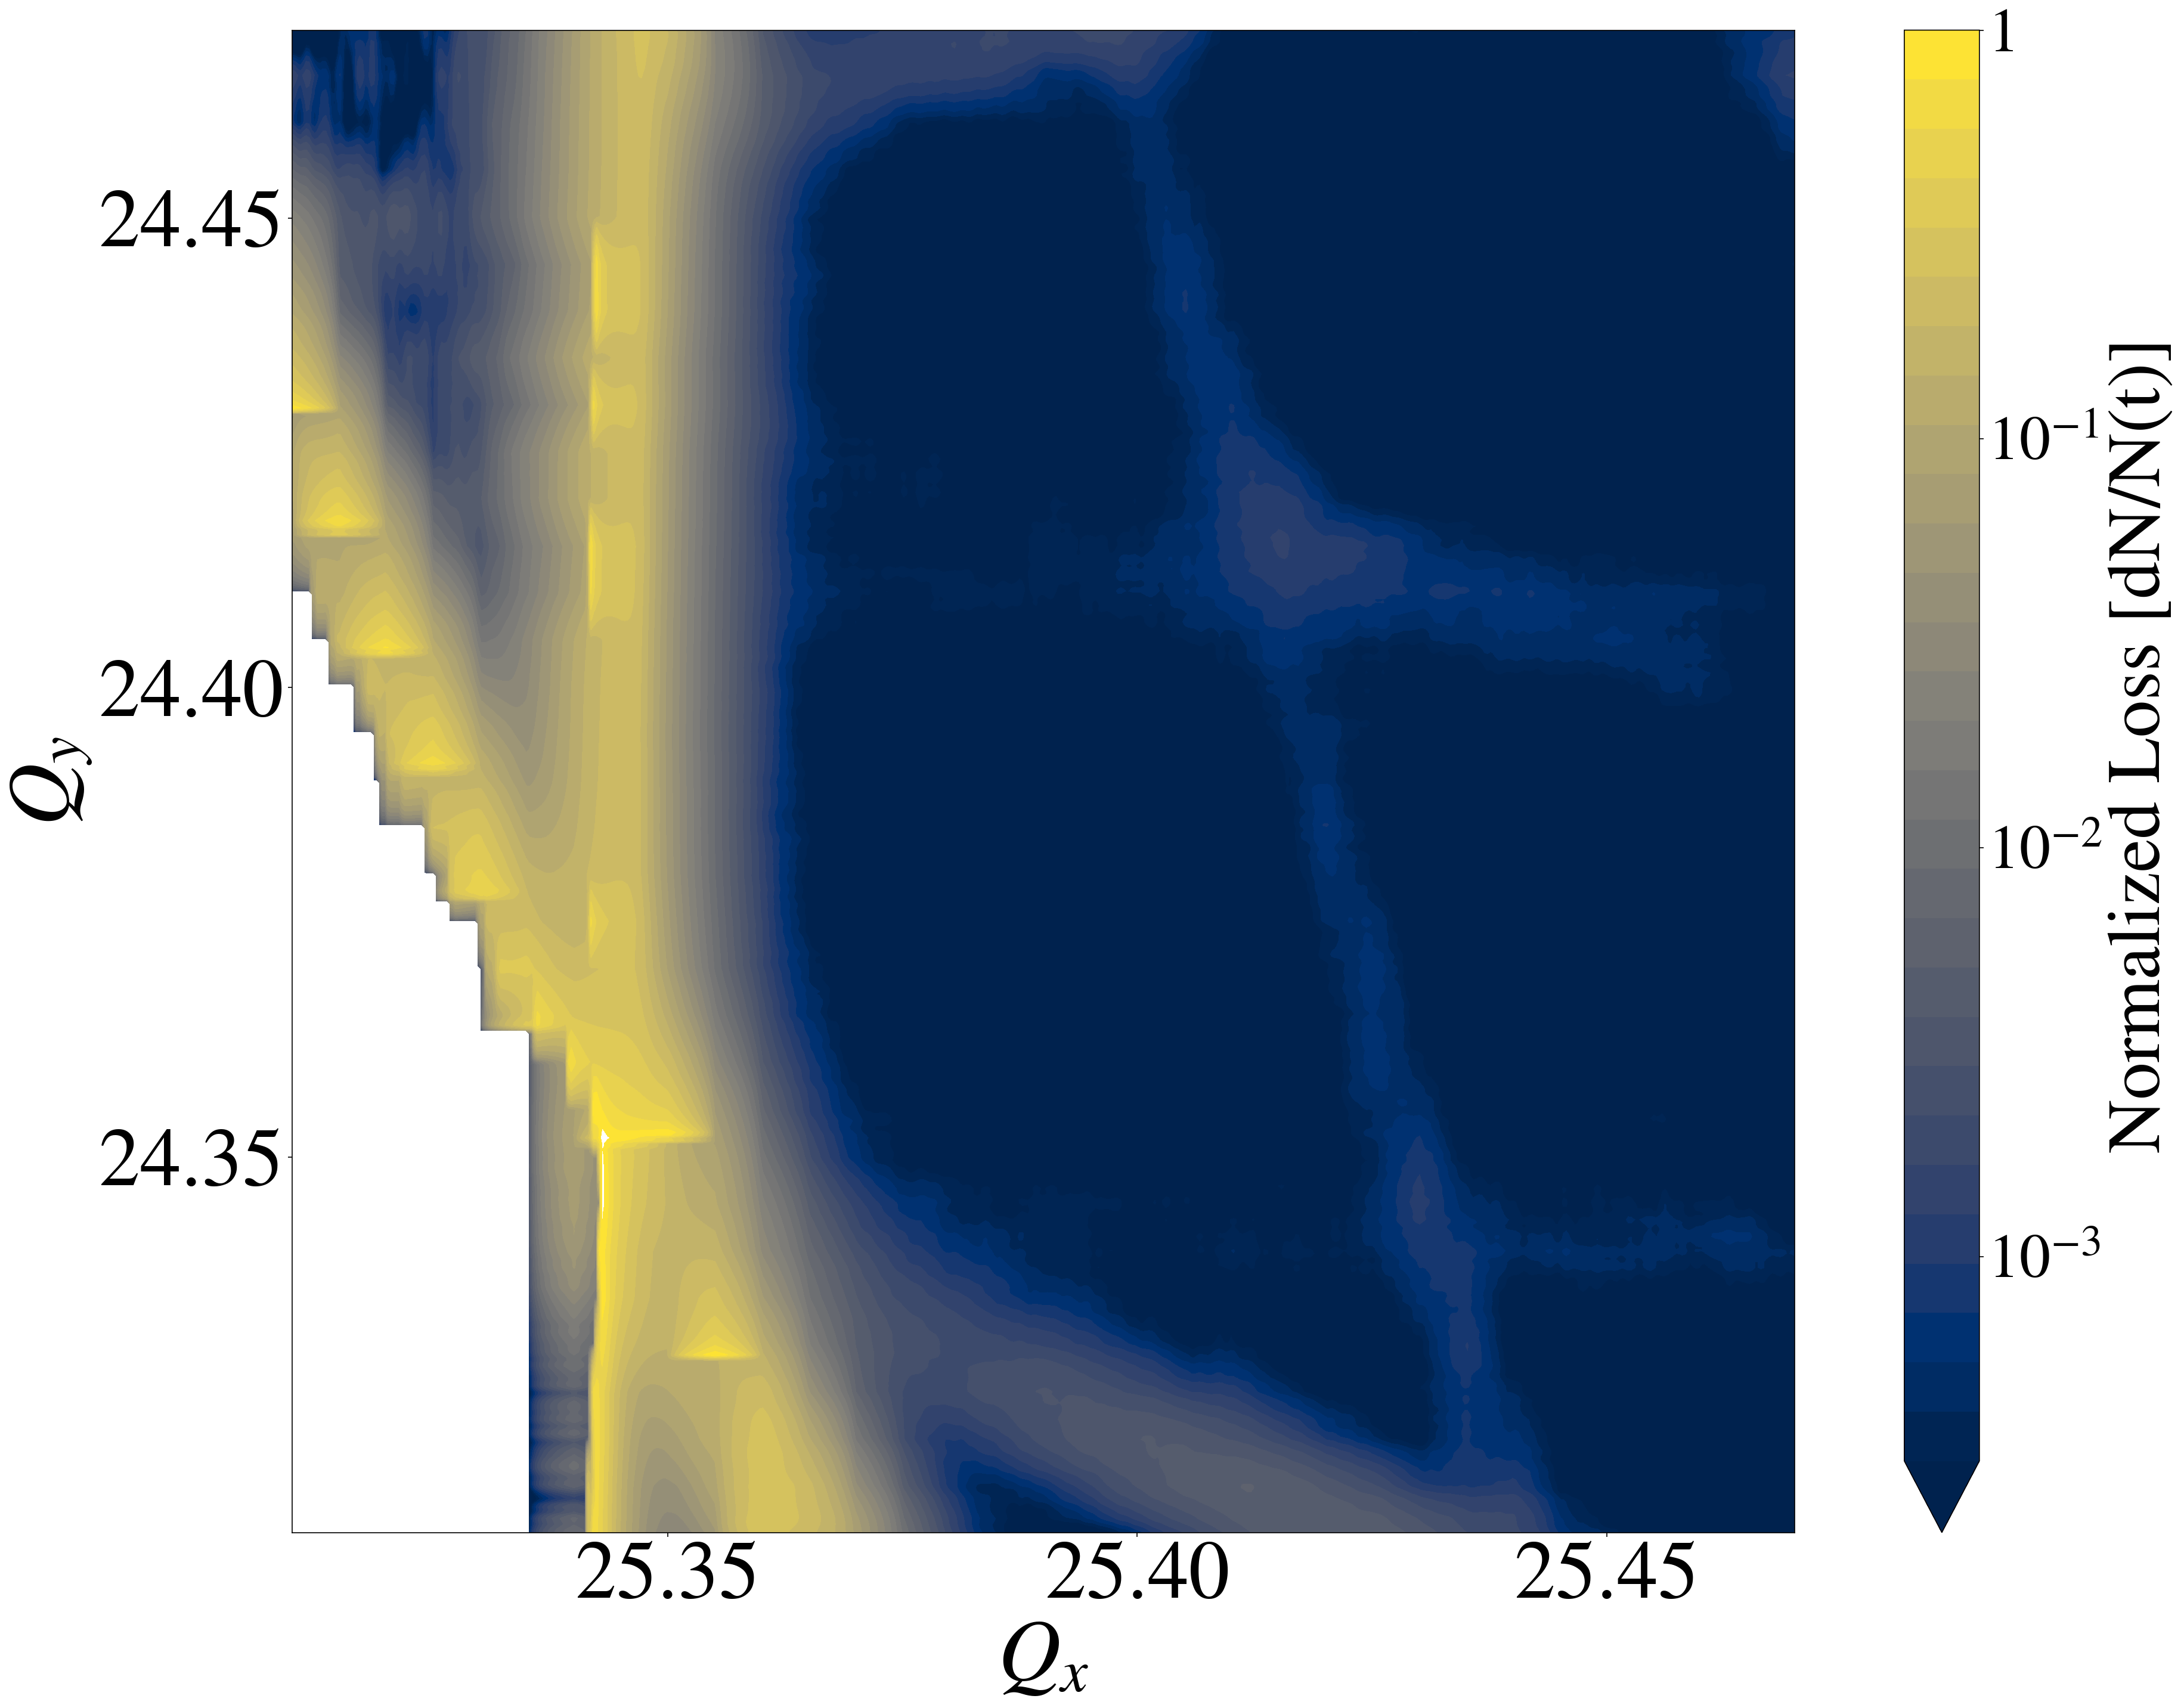
\includegraphics[width=0.98\linewidth]{chapter4/3qy_qx2qy.png}
      \caption{$3Q_y$ and $Q_x+2Q_y$ Compensation}
      \label{fig:sfig6}
    \end{subfigure}
    
    \caption{Dynamic loss maps for several configurations of compensation sextupoles}
    \label{fig:lossmaps}
    \end{figure} 
\newpage


\subsection{Static Tune Scans}

\begin{figure}[H]
    \centering
    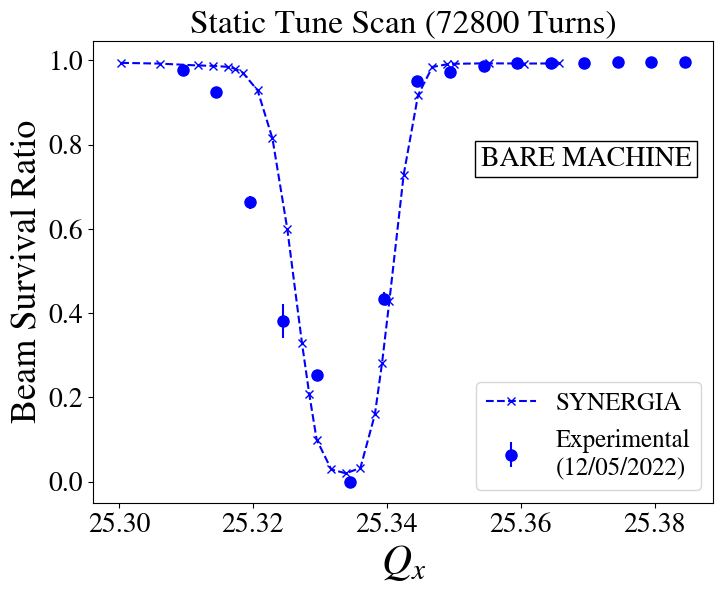
\includegraphics[width=\columnwidth]{chapter4/static2turns.png}
    \caption{Static tune scan for bare machine with comparisons between experimental data and SYNERGIA simulations.}
    \label{fig:static2}
\end{figure}

\begin{figure}[H]
    \centering
    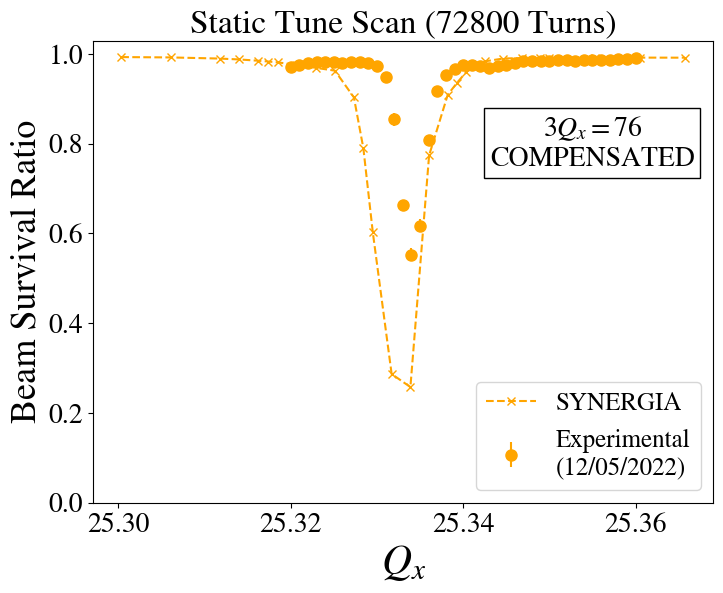
\includegraphics[width=\columnwidth]{chapter4/static2turns_comp.png}
    \caption{Plot for static tune scan for machine with $3Q_x$ compensation including comparison between experimental data and SYNERGIA simulations.}
    \label{fig:static2_comp}
\end{figure}